%===============================================================================
% LaTeX sjabloon voor de bachelorproef toegepaste informatica aan HOGENT
% Meer info op https://github.com/HoGentTIN/latex-hogent-report
%===============================================================================

\documentclass[dutch,dit,thesis]{hogentreport}

% \usepackage{lipsum} % For blind text, can be removed after adding actual content

%% Pictures to include in the text can be put in the graphics/ folder
\graphicspath{{graphics/}}

%% For source code highlighting, requires pygments to be installed
%% Compile with the -shell-escape flag!
%% \usepackage[chapter]{minted}
%% If you compile with the make_thesis.{bat,sh} script, use the following
%% import instead:
%%\usepackage[chapter,outputdir=../output]{minted}
\usepackage[chapter]{minted}
\usemintedstyle{solarized-light}

%% Formatting for minted environments.
\setminted{%
    autogobble,
    frame=lines,
    breaklines,
    linenos,
    tabsize=4
}

%% Ensure the list of listings is in the table of contents
\renewcommand\listoflistingscaption{%
    \IfLanguageName{dutch}{Lijst van codefragmenten}{List of listings}
}
\renewcommand\listingscaption{%
    \IfLanguageName{dutch}{Codefragment}{Listing}
}
\renewcommand*\listoflistings{%
    \addcontentsline{toc}{chapter}{\listoflistingscaption}%
    \listof{listing}{\listoflistingscaption}%
}

%% For source code highlighting, requires pygments to be installed
%% Compile with the -shell-escape flag!
%%\usepackage[chapter]{minted}
\usepackage{caption}
\usepackage{subcaption}

%% Change this line to edit the line numbering style:
\renewcommand{\theFancyVerbLine}{\ttfamily\scriptsize\arabic{FancyVerbLine}}

%% Macro definition to load external python source files with \pythoncode{filename}:
% \newmintedfile[pythoncode]{python}{
%     bgcolor=bg,
%     fontfamily=tt,
%     linenos=true,
%     numberblanklines=true,
%     numbersep=5pt,
%     gobble=0,
%     framesep=2mm,
%     funcnamehighlighting=true,
%     tabsize=4,
%     obeytabs=false,
%     breaklines=true,
%     mathescape=false
%     samepage=false,
%     showspaces=false,
%     showtabs =false,
%     texcl=false,
% }

% Other packages not already included can be imported here

%%---------- Document metadata -------------------------------------------------
% TODO: Replace this with your own information
\author{Max Milan}
\supervisor{Dhr. G. Bosteels}
\cosupervisor{Dhr. A. Pannemans}
\title%[Optionele ondertitel]%
    {Geautomatiseerde documentatie generatie met behulp van Large Language Modellen: Het genereren van duidelijke overzichten en informatieve beschrijvingen voor ongedocumenteerde Python-projecten}
\academicyear{\advance\year by -1 \the\year--\advance\year by 1 \the\year}
\examperiod{1}
\degreesought{\IfLanguageName{dutch}{Professionele bachelor in de toegepaste informatica}{Bachelor of applied computer science}}
\partialthesis{false} %% To display 'in partial fulfilment'
%\institution{Internshipcompany BVBA.}

%% Add global exceptions to the hyphenation here
\hyphenation{back-slash}

%% The bibliography (style and settings are  found in hogentthesis.cls)
\addbibresource{bachproef.bib}            %% Bibliography file
\addbibresource{../voorstel/voorstel.bib} %% Bibliography research proposal
\defbibheading{bibempty}{}

%% Prevent empty pages for right-handed chapter starts in twoside mode
\renewcommand{\cleardoublepage}{\clearpage}

\renewcommand{\arraystretch}{1.2}

%% Content starts here.
\begin{document}

%---------- Front matter -------------------------------------------------------

\frontmatter

\hypersetup{pageanchor=false} %% Disable page numbering references
%% Render a Dutch outer title page if the main language is English
\IfLanguageName{english}{%
    %% If necessary, information can be changed here
    \degreesought{Professionele Bachelor toegepaste informatica}%
    \begin{otherlanguage}{dutch}%
       \maketitle%
    \end{otherlanguage}%
}{}

%% Generates title page content
\maketitle
\hypersetup{pageanchor=true}

%%=============================================================================
%% Voorwoord
%%=============================================================================

\chapter*{\IfLanguageName{dutch}{Woord vooraf}{Preface}}%
\label{ch:voorwoord}

%% TODO:
%% Het voorwoord is het enige deel van de bachelorproef waar je vanuit je
%% eigen standpunt (``ik-vorm'') mag schrijven. Je kan hier bv. motiveren
%% waarom jij het onderwerp wil bespreken.
%% Vergeet ook niet te bedanken wie je geholpen/gesteund/... heeft

Toen ik aan de richting Toegepaste Informatica begon, wist ik meteen welke specialisatie ik wilde volgen: AI en Data Engineering sprak mij direct aan. 
Deze richting biedt mij de mogelijkheid om steeds nieuwe uitdagingen te vinden in alles wat ik doe.

Het hebben van een uitdaging geeft mij de motivatie om steeds het beste van mezelf te geven. 
Zo was het ook een uitdaging om deze bachelorproef tot een goed einde te brengen. 
Een van de grootste uitdagingen was het werken met LLM's, aangezien dit de eerste keer was dat ik deze zelf implementeerde.

Daarom wil ik graag mijn co-promotor, Arne Pannemans, bedanken voor zijn onophoudelijke steun en waardevolle bijdragen. 
Uw voortdurende aanwezigheid bij het geven van feedback en uw kritische blik waren van onschatbare waarde voor het tot stand brengen van deze bachelorproef. 
Uw continue steun en toewijding hebben mij geïnspireerd en gemotiveerd om het beste uit mezelf te halen. 
Dankzij uw begeleiding heb ik mijn onderzoek naar een hoger niveau kunnen tillen.

Ook wil ik mijn promotoren meneer Gert-Jan Bosteels en mevrouw Lena De Mol bedanken voor hun kritische en waardevolle feedback. 
Deze feedback heeft ervoor gezorgd dat ik de juiste richting uitging en dat ik mijn ideeën helder kon verwoorden.

Tot slot zou ik graag mijn ouders en vrienden willen bedanken. Hun steun, voortdurende aanmoediging en begrip hebben mij door alle moeilijke momenten geholpen. 
Dankzij hen heb ik deze bachelorproef tot een goed einde kunnen brengen.

%%=============================================================================
%% Samenvatting
%%=============================================================================

% TODO: De "abstract" of samenvatting is een kernachtige (~ 1 blz. voor een
% thesis) synthese van het document.
%
% Een goede abstract biedt een kernachtig antwoord op volgende vragen:
%
% 1. Waarover gaat de bachelorproef?
% 2. Waarom heb je er over geschreven?
% 3. Hoe heb je het onderzoek uitgevoerd?
% 4. Wat waren de resultaten? Wat blijkt uit je onderzoek?
% 5. Wat betekenen je resultaten? Wat is de relevantie voor het werkveld?
%
% Daarom bestaat een abstract uit volgende componenten:
%
% - inleiding + kaderen thema
% - probleemstelling
% - (centrale) onderzoeksvraag
% - onderzoeksdoelstelling
% - methodologie
% - resultaten (beperk tot de belangrijkste, relevant voor de onderzoeksvraag)
% - conclusies, aanbevelingen, beperkingen
%
% LET OP! Een samenvatting is GEEN voorwoord!

%%---------- Samenvatting -----------------------------------------------------
% De samenvatting in de hoofdtaal van het document

\chapter*{\IfLanguageName{dutch}{Samenvatting}{Abstract}}

Deze bachelorproef richt zich op het documenteren van ongedocumenteerde\\ Python-projecten met behulp van een Large Language Model (LLM).
Het genereren van duidelijk en overzichtelijke documentatie van een project helpt bij het begrijpen van de code en is de eerste stap in het delen van kennis.
Bestaande tools hebben echter gedocumenteerde code nodig om documentatie te genereren. 
Het automatiseren van het documentatieproces zorgt ervoor dat dit geen manuele taak meer is.  

De centrale onderzoeksvraag is: "Hoe kan geautomatiseerde documentatiegeneratie met behulp van Large Language Modellen (LLM) effectief worden toegepast op ongedocumenteerde Python-projecten om er duidelijke en overzichtelijke documentatie van te maken?" 
Deze vraag is verder opgesplitst in enkele deelvragen, wat is documentatie en wat is er nodig om een bestand en een project te documenteren?
Met als doel een Proof of Concept (PoC) van een geautomatiseerde tool die de code van een Python-project analyseert en er documentatie van genereert.

Het onderzoek omvat enkele fases. Eerst wordt er gekeken hoe een enkel bestand gedocumenteerd kan worden. 
Vervolgens wordt er gekeken hoe verschillende bestanden in een project samen gedocumenteerd kunnen worden om zo een overzicht van het project te geven.
De laatste fase beslaagt het evalueren van de tool door de documentatie van de tool te vergelijken met de handgeschreven documentatie van een project.

De resultaten van de evaluatie tonen aan dat de documentatie van de tool en de handgeschreven documentatie gelijkaardig zijn en door de visuele weergave van de relaties tussen de bestanden is de documentatie overzichtelijk en duidelijk.
Er kunnen echter wel enkele fouten in de documentatie sluipen.

Deze studie biedt een oplossing voor het documenteren van ongedocumenteerde Python-projecten en kan gebruikt worden om de kennis van een project te delen met anderen.


%---------- Inhoud, lijst figuren, ... -----------------------------------------

\tableofcontents

% In a list of figures, the complete caption will be included. To prevent this,
% ALWAYS add a short description in the caption!
%
%  \caption[short description]{elaborate description}
%
% If you do, only the short description will be used in the list of figures

\listoffigures
\listoftables
\listoflistings

% If you included tables and/or source code listings, uncomment the appropriate
% lines.

% Als je een lijst van afkortingen of termen wil toevoegen, dan hoort die
% hier thuis. Gebruik bijvoorbeeld de ``glossaries'' package.
% https://www.overleaf.com/learn/latex/Glossaries

%---------- Kern ---------------------------------------------------------------

\mainmatter{}

% De eerste hoofdstukken van een bachelorproef zijn meestal een inleiding op
% het onderwerp, literatuurstudie en verantwoording methodologie.
% Aarzel niet om een meer beschrijvende titel aan deze hoofdstukken te geven of
% om bijvoorbeeld de inleiding en/of stand van zaken over meerdere hoofdstukken
% te verspreiden!

%%=============================================================================
%% Inleiding
%%=============================================================================

\chapter{\IfLanguageName{dutch}{Inleiding}{Introduction}}%
\label{ch:inleiding}

De inleiding moet de lezer net genoeg informatie verschaffen om het onderwerp te begrijpen en in te zien waarom de onderzoeksvraag 
de moeite waard is om te onderzoeken. In de inleiding ga je literatuurverwijzingen beperken, zodat de tekst vlot leesbaar blijft. 
Je kan de inleiding verder onderverdelen in secties als dit de tekst verduidelijkt. 
Zaken die aan bod kunnen komen in de inleiding~\autocite{Pollefliet2011}:

\begin{itemize}
  \item context, achtergrond
  \item afbakenen van het onderwerp
  \item verantwoording van het onderwerp, methodologie
  \item probleemstelling
  \item onderzoeksdoelstelling
  \item onderzoeksvraag
  \item \ldots
\end{itemize}

\section{\IfLanguageName{dutch}{Probleemstelling}{Problem Statement}}%
\label{sec:probleemstelling}

Projecten worden vaak niet goed gedocumenteerd, dit kan leiden tot problemen in de toekomst. Wanneer een andere persoon de code van een ongedocumenteerd project wilt gebruiken moet de code volledig gelezen worden voordat er begrepen wordt wat de code doet. 
Dit is een tijdrovend proces en kan voorkomen worden door goede documentatie.
Wanneer de code jaren later aangepast moet worden is het ook handig om goede documentatie te hebben, zodat de persoon weet waar er aanpassingen moeten gebeuren.
De skills en know-how van een project kunnen verloren gaan wanneer er geen documentatie is.
Deze dienen juist gedeeld te worden met anderen zodat er geen dubbel werk gedaan moet worden.
Het is dus belangrijk dat er aan documentatie gedaan wordt en dat deze up-to-date blijft.

Het documenteren van een project is iets wat veel tijd kost en wat meestal geen aandacht krijgt.
Een tool die dit proces kan versnellen / automatiseren zou een grote meerwaarde zijn.
De tool bestaat uit een geautomatiseerde documentatie LLM die de project code analyseert en samenvat in een document. 
Dit geeft de lezers de mogelijkheid om zich in te lezen in het project en erna zelf aanpassingen te maken of stukken code te gebruiken voor een ander project.

\section{\IfLanguageName{dutch}{Onderzoeksvraag}{Research question}}%
\label{sec:onderzoeksvraag}

Hoe kan geautomatiseerde documentatiegeneratie met behulp van Large Language Modellen (LLM) effectief worden toegepast om duidelijke en informatieve overzichten te produceren voor Python projecten?

\section{\IfLanguageName{dutch}{Onderzoeksdoelstelling}{Research objective}}%
\label{sec:onderzoeksdoelstelling}

Het eindresultaat van deze bachelorproef is een Proof of Concept (PoC) van een geautomatiseerde tool die de project code analyseert en er documentatie van genereert.
De gegenereerde documentatie laat het toe het project te begrijpen zonder er te veel tijd aan te besteden.

\section{\IfLanguageName{dutch}{Opzet van deze bachelorproef}{Structure of this bachelor thesis}}%
\label{sec:opzet-bachelorproef}

% Het is gebruikelijk aan het einde van de inleiding een overzicht te
% geven van de opbouw van de rest van de tekst. Deze sectie bevat al een aanzet
% die je kan aanvullen/aanpassen in functie van je eigen tekst.

De rest van deze bachelorproef is als volgt opgebouwd:

In Hoofdstuk~\ref{ch:stand-van-zaken} wordt een overzicht gegeven van de stand van zaken binnen het onderzoeksdomein, op basis van een literatuurstudie.

In Hoofdstuk~\ref{ch:methodologie} wordt de methodologie toegelicht en worden de gebruikte onderzoekstechnieken besproken om een antwoord te kunnen formuleren op de onderzoeksvragen.

% TODO: Vul hier aan voor je eigen hoofstukken, één of twee zinnen per hoofdstuk

In Hoofdstuk~\ref{ch:conclusie}, tenslotte, wordt de conclusie gegeven en een antwoord geformuleerd op de onderzoeksvragen. Daarbij wordt ook een aanzet gegeven voor toekomstig onderzoek binnen dit domein.
\chapter{\IfLanguageName{dutch}{Stand van zaken}{State of the art}}%
\label{ch:stand-van-zaken}

% Tip: Begin elk hoofdstuk met een paragraaf inleiding die beschrijft hoe
% dit hoofdstuk past binnen het geheel van de bachelorproef. Geef in het
% bijzonder aan wat de link is met het vorige en volgende hoofdstuk.

% Pas na deze inleidende paragraaf komt de eerste sectiehoofding.

In dit hoofdstuk wordt de literatuurstudie besproken. 
Door deze literatuurstudie is het mogelijk om een beter inzicht te krijgen in de technologie en mogelijkheden voor de documentatie van Python-projecten alsook hoe het toegepast kan worden met behulp van Large Language Modellen. 
Er zal nadruk worden gelegd op bestaande literatuur en onderzoeken die verbonden zijn met documentatie van Python-projecten. 
In dit onderdeel zullen verschillende hoofdstukken worden aangekaart. 
Als eerste zal er duidelijk gemaakt worden wat er juist verstaan wordt onder documentatie. 
Vervolgens wordt er gekeken naar bestaande documentatie tools.
In het derde deel van deze literatuurstudie wordt er gekeken wat Large Language Modellen zijn, hoe deze werken en wat enkele bestaande modellen zijn.

\section{Wat is documentatie?}
\label{sec:wat-is-documentatie}

Alvorens dieper op het onderwerp in te gaan, is het belangrijk dat er een duidelijk beeld gevormd wordt wat documentatie is. 
Waarom is documentatie belangrijk voor een project en wat wordt er begrepen onder documentatie? 

Documentatie is het proces van het vastleggen van de werking van een project.
Volgens \textcite{CodeQuality2024} kan dit op verschillende manieren gebeuren. 
Er kan gekozen worden om de documentatie te schrijven in de vorm van een commentaar in de code, een docstring, een API voor klassen of functies of in de vorm van een README.md bestand \autocite{CodeQuality2024}.
Het doel van documentatie is om de werking van het project te beschrijven zodat andere programmeurs het project kunnen begrijpen en gebruiken.
Zo gaat er geen tijd verloren aan het lezen van de code en het begrijpen ervan.

Documentatie kan gemaakt worden voor verschillende doelgroepen. Het kan voor interne of externe doeleinden zijn.
Interne documentatie is voor documentatie binnen hetzelfde bedrijf.
Dit gaat dan om het capteren van de proces kennis die vergaard is binnen een project. Dit is informatie zoals een roadmap of product requirements. 
Deze documentatie gaat over het vastleggen van gedetaïlleerde uitleg over hoe iets werkt en hoe het onderhouden kan worden \autocite{swimm.io2024}.

Externe documentatie is voor documentatie die gedeeld wordt met andere bedrijven of klanten. 
Dit gaat dan over de basiswerking van de code van een project zodat andere programmeurs het kunnen gebruiken.
Gebruiksaanwijzingen of handleidingen zijn ook een vorm van externe documentatie \autocite{swimm.io2024}.

Voor deze bachelorproef wordt er gekeken naar het documenteren van een Python-project in de vorm van commentaar in de code en het genereren van een samenvattend document van het gehele project.
Omdat Python een populaire programmeertaal is volgens \textcite{TIOBE2024} en er veel projecten in deze taal geschreven worden, is het interessant om te kijken hoe deze projecten gedocumenteerd kunnen worden.
Ook kan er in de code bij functies aan type hinting gedaan worden. Dit indiceert wat de datatypes van de input en output van een functie zijn \autocite{Bailey2024}.
Uit deze documentatie kan de werking van het project duidelijk worden en kunnen de relaties tussen de verschillende bestanden en functies weergegeven worden.

In het verdere verloop van deze bachelorproef wordt er gekeken hoe de documentatie van een Python-project gegenereerd kan worden.

\subsection{Bestand documentatie}
\label{sec:bestand-documentatie}
Eerst dienen de bestanden van het project gedocumenteerd te worden.
Dit gebeurt door de code van het bestand te analyseren en de docstrings van de verschillende functies en klassen te genereren.

Docstrings of documentatie strings worden aan het begin van een functie of klasse geplaatst.
Deze strings worden gebruikt om de functie of klasse te documenteren \autocite{GeeksforGeeks2023}.
Volgens \textcite{GeeksforGeeks2023} zijn docstrings vitaal in het overdragen van het doel en de werking van een functie of klasse.

Deze docstrings kunnen dan gebruikt worden om een samenvatting van het bestand te genereren.

\subsection{Project documentatie}
\label{sec:project-documentatie-literatuur}
De documentatie van het project wordt gemaakt door de samenvattingen van de verschillende bestanden te combineren.
Deze samenvattingen worden gegenereerd op basis van de samenvatting van de bestanden die tot het project behoren.
In deze samenvatting behoort de werking van het project, de verschillende bestanden met functies en klassen en de relaties tussen deze bestanden.


\section{Bestaande documentatie tools}
\label{sec:huidige-tools}
Voor er gekeken wordt hoe LLM's mogelijk gebruikt kunnen worden voor het genereren van documentatie is het belangrijk dat er een helder beeld is van de huidige tools die gebruikt worden voor het genereren van documentatie.
De documentatie kan in verschillende vormen gegeneerd worden. Dit kan gaan van een website tot een samenvattend document.
Ook kunnen er in de code zelf commentaren geplaatst worden die de werking van de code uitleggen.
Hiervoor bestaan er reeds verschillende tools en dit voor verschillende programmeertalen opgelijst in tabel \ref{table:vgl-tools}.
In dit onderdeel is er enkel gekeken naar tools die nog onderhouden worden door de makers. 

\subsection{Doxygen}
Doxygen \autocite{Doxygen2023} is een tool die het toelaat om automatisch code documentatie te genereren. Het is een gratis tool die bruikbaar is voor verschillende programmeertalen zoals: C++, C, Python, PHP en Java.
Het genereert documentatie in de vorm van HTML, LaTeX, RT. 
Deze tool is in staat om een diagram te genereren met de relaties tussen de verschillende delen van de code bijvoorbeeld de relaties tussen de verschillende klassen en functies.
Een voorbeeld van een diagram kan gezien worden in figuur \ref{fig:Doxygen-diagram}.
Zo wordt er een duidelijk beeld verkregen van de structuur van het project.

\begin{figure}[h]
  \centering
  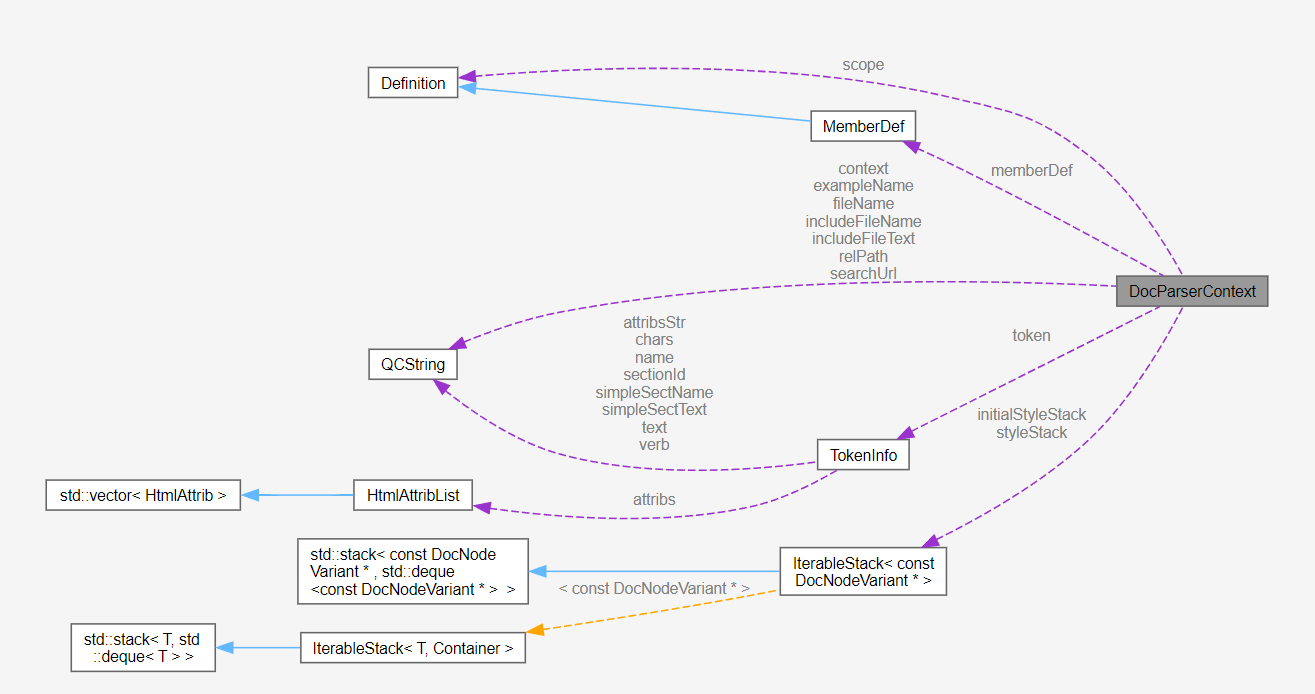
\includegraphics[width=1\textwidth]{doxygen_diagram.png}
  \caption{Voorbeeld diagram van Doxygen \autocite{Doxygen2023}}
  \label{fig:Doxygen-diagram}
\end{figure}

\subsection{CodeCat}
\textcite{CodeCat2024} is een online tool die de code analyseert en de docstrings genereert. Er kan niet gekeken worden naar de werking van CodeCat aangezien het niet open sourced is.
Deze tool genereert automatisch de docstrings voor JavaScript code.

\subsection{GPT4Docstrings}
De tool van \textcite{Trofficus2023} genereert docstrings voor Python code. Het maakt gebruik van GPT-4 \autocite{OpenAI2023} om de docstrings te genereren.
Deze tool leunt sterk aan bij de doelstelling van deze bachelorproef, namelijk het genereren van documentatie met behulp van LLM's.
Het nader bekijken van deze tool kan een meerwaarde zijn voor deze bachelorproef.

\begin{figure}
  \centering
  \begin{subfigure}[b]{0.5\textwidth}
      \centering
      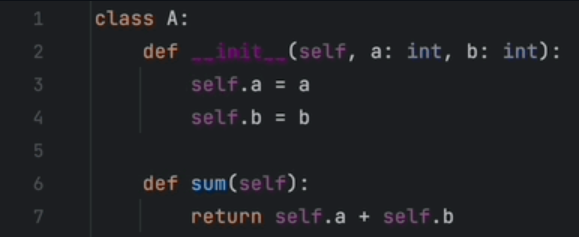
\includegraphics[width=1\textwidth]{before_troficus.png}
      \caption{Voorbeeld code zonder docstrings van \textcite{Trofficus2023}}
      \label{fig:before-Trofficus}
  \end{subfigure}
  \hfill
  \begin{subfigure}[b]{0.5\textwidth}
      \centering
      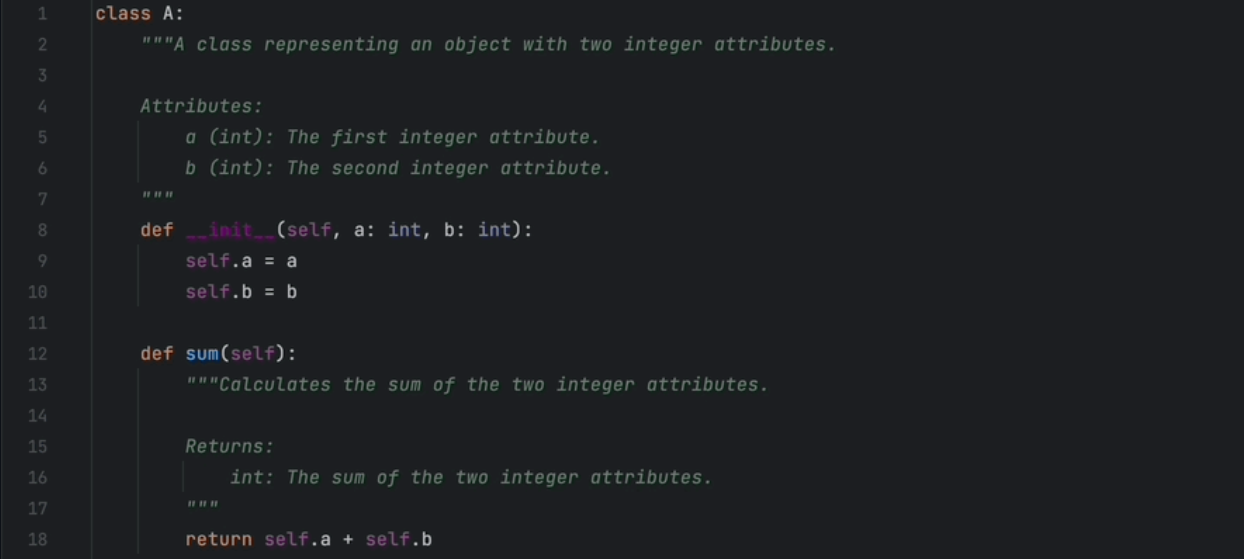
\includegraphics[width=1\textwidth]{after_troficus.png}
      \caption{Voorbeeld code met docstrings van \textcite{Trofficus2023}}
      \label{fig:after-Trofficus}
  \end{subfigure}
     \caption[Uitkomst GPT4Docstrings]{Voorbeeld uitkomst van de tool van \textcite{Trofficus2023}}
     \label{fig:Before-After-Trofficus}
\end{figure}

Zo gebruikt GPT4Docstrings van \textcite{Trofficus2023} de Abstract Syntax Tree (AST) van de code om de structuur van de code te begrijpen.
Uit de AST kunnen de juiste stukken code gehaald worden om de docstrings te genereren.
Dit kan goed van pas komen voor het genereren van documentatie van Python-projecten.
Een voorbeeld van deze tool kan gezien worden in figuur \ref{fig:Before-After-Trofficus}. 

\subsection{Sphinx}
Sphinx van \textcite{Sphinx2023} is één van de meest gebruikte tools voor het genereren van documentatie voor Python-projecten.
Het genereert documentatie aan de hand van docstrings. Het toont de hiërarchie van het project om een duidelijk overzicht te geven.
Deze tool is vrij flexibel want het kan uitgebreid worden met verschillende extensies, zodat het alle mogelijke wensen kan vervullen.
Volgens \textcite{Sphinx2023} kan de extensie autodoc semi-automatisch de docstrings van een module extraheren en in de documentatie plaatsen. 
Dit is handig wanneer de automatische documentatie generatie van een geheel project gewenst is. Zo kan het project samengevat worden aan de hand van de docstrings van de verschillende python files. 
Alvorens een Python-project gedocumenteerd kan worden met Sphinx \autocite{Sphinx2023} dienen alle bestanden aangevuld te worden met docstrings.
Dit gebeurt echter niet bij het runnen van het programma.

\subsection{Pdoc}
Pdoc \autocite{GallantHils2023} genereert documentatie in de vorm van een website die een API van de documentatie bevat. 
Hier kan er eenvoudig op de website gezocht worden naar een functie of klasse met de bijhorende documentatie.

\begin{table}[h!]
\centering
\resizebox{\textwidth}{!}{
\begin{tabular}{|c|c|c|}
\hline
Tool & programmeertaal & type \\ [0.5ex]
\hline
Doxygen & C++, C, Python, PHP, Java & HTML, PDF, markdown\\
\hline
CodeCat & JavaScript & docstring \\
\hline
Sphinx & Python & HTML, LATEX, man pages \\
\hline
Pdoc & Python & API \\
\hline
GPT4Docstrings & Python & docstring \\
\hline
\end{tabular}}
\caption{Vergelijking documentatie tools}
\label{table:vgl-tools}
\end{table}

\subsection{Samenvatting tools}
\label{sec:samenvatting-tools}
Door de verschillende tools op te lijsten en te vergelijken met elkaar wordt er een duidelijk beeld gevormd wat de tools kunnen genereren.
Zo kan er een keuze gemaakt worden welke tool het beste past bij dit onderzoek.
In tabel \ref{table:ra-tools} wordt er een overzicht gegeven wat de tools kunnen genereren.
De tools Doxygen, Sphinx en Pdoc kunnen enkel een document genereren in de vorm van een website of een bestand op basis van reeds bestaande docstrings en commentaren in de code.
De tool GPT4Docstrings genereert docstrings voor Python code met behulp van een LLM.

\begin{table}[h!]
  \centering
  \resizebox{\textwidth}{!}{
  \begin{tabular}{|c|c|c|c|c|}
  \hline
  Tool & docstrings & samenvatting bestand & samenvatting project & visualisatie \\ [0.5ex]
  \hline
  GPT4Docstrings & ja & nee & nee & nee \\
  \hline
  Doxygen & nee & nee & nee & ja \\
  \hline
  Sphinx & nee & nee & nee & nee \\
  \hline
  Pdoc & nee & nee & nee & nee \\
  \hline
  \end{tabular}}
  \caption{Overzicht van wat de tools kunnen genereren}
  \label{table:ra-tools}
  \end{table}

\section{Wat zijn Large Language Modellen (LLM)?}
\label{sec:wat-zijn-llms}

Uit de vorige sectie is gebleken dat er slechts één tool geschikt is voor het genereren van documentatie voor projecten zonder gedocumenteerde code. 
De tool GPT4Docstrings van \textcite{Trofficus2023} maakt gebruik van een Large Language Model (LLM) om de docstrings te genereren.
Het is dus belangrijk dat er een duidelijk beeld is van wat LLM's juist zijn en hoe deze werken.
Wat kunnen deze modellen, wat zijn de mogelijke beperkingen en wat is de huidige stand van zaken. 
In dit hoofdstuk wordt er een antwoord gegeven op de vragen: 
\begin{itemize}
  \item Bestaan er LLM's speciaal getraind op Python code? 
  \item Kunnen LLM's gebruikt worden om documentatie te genereren?
\end{itemize}

Dit draagt bij tot het verkrijgen van een grondige basiskennis van LLM's. 
Het veld waarin AI zich bevindt, wordt vaak voorgesteld volgens figuur \ref{fig:LLM-position}. Het bestaat uit verschillende cirkels met elk een eigen laag volgens \textcite{Stoeffelbauer2023}.
Deze lagen zijn: Artificiële Intelligentie, Machine Learning, Deep Learning en Large Language Modellen.
Omdat LLM's een subveld zijn van Deep Learning is het belangrijk dat er een duidelijk beeld is van wat Deep Learning juist is.
Uit de figuur \ref{fig:LLM-position} blijkt dat AI verschillende categorieën omvat.
Volgens \textcite{Stoeffelbauer2023} is AI een brede term wat vaak verwijst naar slimme machines. 
Machine Learning (ML) is een subveld van AI, waarin patronen worden herkend tussen een input en een output.
ML kan gebruikt worden voor verschillende taken zoals classificatie, regressie, clustering en dergelijke.
Volgens \textcite{Stoeffelbauer2023} is Deep Learning (DL) een subveld van ML, waarin complexe algoritmen en Deep Neural Networks gebruikt worden om complexere taken uit te voeren.
Deep Learning is een krachtige tool die gebruikt wordt voor verschillende taken zoals: beeldherkenning, spraakherkenning, ...

\begin{figure}[h]
  \centering
  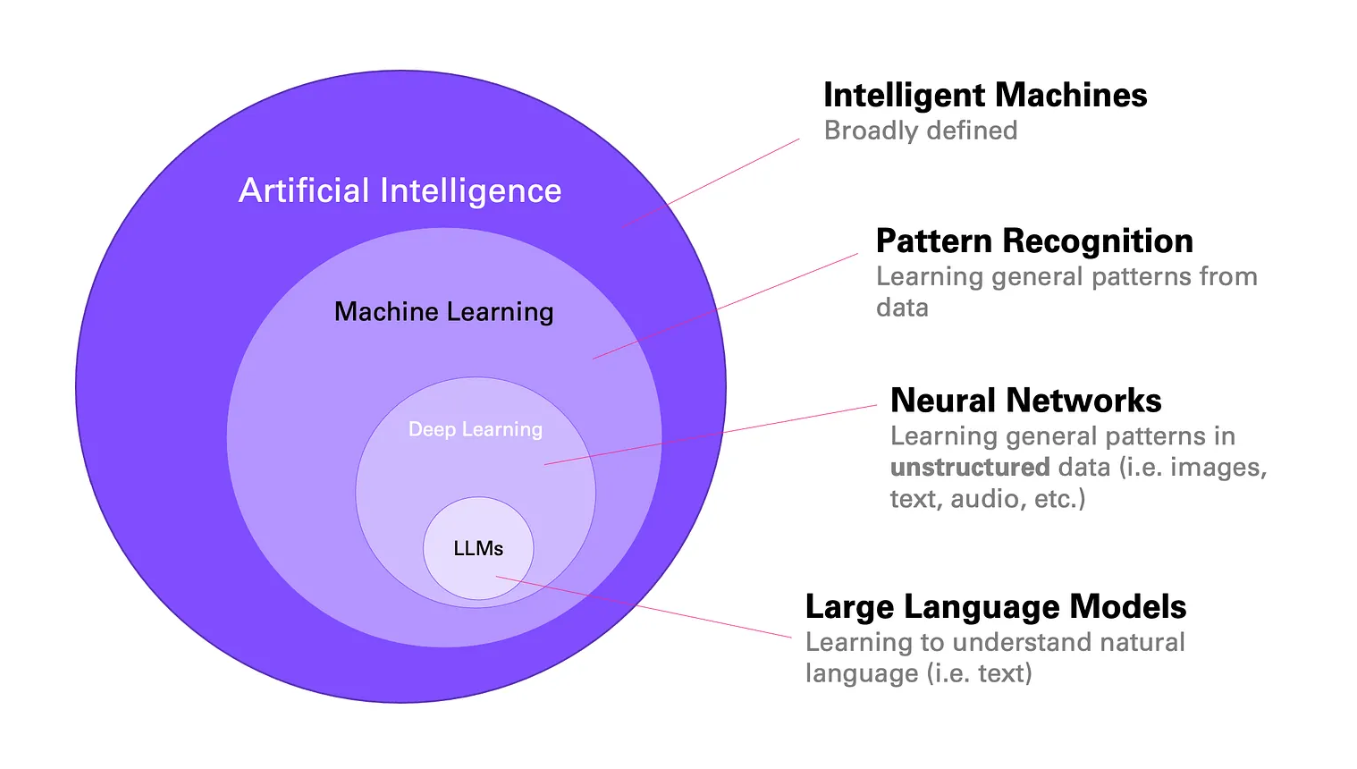
\includegraphics[width=0.5\textwidth]{LLMsphere.png}
  \caption{Artificiële intelligentie in lagen \autocite{Stoeffelbauer2023}}
  \label{fig:LLM-position}
\end{figure}

Large Language Modellen zijn geavanceerde AI-systemen die dienen om menselijke taal te verstaan, te genereren en te verwerken.
LLM's worden getraind op een grote hoeveelheid tekst wat vaak uit allerlei data zoals artikels of websites gehaald wordt. 
Volgens \textcite{Beelen2023} zorgen Deep Neural Networks ervoor dat LLM's natuurlijke taal verwerken op een gelijkaardige manier die vergelijkbaar is met de menselijke taalvaardigheid.
Deze hebben een grote vooruitgang gekend in 2017 door de paper van \textcite{VaswaniEtAl2017}. 
Hieruit kwam een nieuw mechanisme tot stand namelijk transformers wat bestaat uit Attentie blokken. 
Enkele voordelen die komen kijken bij het gebruiken van transformers zijn: 
\begin{itemize}
  \item Het kan lange sequenties verwerken.
  \item Het kan parallel sequenties verwerken.
  \item Het kan de relaties tussen de verschillende delen van de sequentie leren.
\end{itemize}
Hierdoor hebben transformer modellen een snellere trainingsperiode dan vorige neurale netwerken \autocite{aiml2023}.

\subsection{Transformers en de architectuur van LLM's}
\label{sec:architectuur-van-llms}
Omdat in dit onderzoek gebruik gemaakt wordt van LLM's is het nodig dat er dieper ingegaan wordt op de architectuur van deze modellen om een beter inzicht te krijgen hoe deze werken.
Een neuraal netwerk bestaat uit verschillende lagen. Enkele belangrijke blokken die gebruikt worden binnen de transformer laag zijn:
\begin{itemize}
  \item Self-Attention
  \item Cross-Attention
  \item Masked Self-Attention
\end{itemize}

Deze Attentie blokken worden gebruikt in de encoder en decoder van een transformer en stromen voort uit het onderzoek van \textcite{VaswaniEtAl2017}.

Transformers zijn een speciaal type van neurale netwerken die gebruik maken van verschillende Attentie blokken.
Attentie is een mechanisme dat gebruikt wordt om de relaties tussen verschillende delen van de invoersequenties te leren.
Een transformer bestaat uit een encoder en een decoder. 
Niet elke transformer bestaat uit zowel een encoder als een decoder het kan ook enkel encoder of decoder bevatten \autocite{Hoque2023}.
De encoder wordt gebruikt om de invoersequenties te verwerken en de decoder wordt gebruikt om de uitvoersequenties te genereren.
Zo is BERT van \textcite{DevlinEtAl2019} een transformer die enkel een encoder heeft en GPT van \textcite{RandfordEtAL2018} heeft enkel een decoder.
De transformer architectuur uit de paper van \textcite{VaswaniEtAl2017} kan gezien worden in figuur \ref{fig:transformer-model}. 

Self-Attention duidt dynamische gewichten toe aan verschillende elementen binnen de meegegeven sequentie, bijvoorbeeld bij woorden in een zin.
Dit laat het model toe om zich te concentreren op de meest relevante delen van de invoer, terwijl de invloed van minder cruciale delen wordt verminderd.
De invoersequentie wordt eerst in drie verschillende vectoren omgezet: Query, Key en Value.
De Query vector stelt een specifiek token uit de invoersequentie voor. De Key vector vertegenwoordigt alle tokens en de vector voor Value bevat de feitelijke inhoud die aan elk token is gekoppeld.
De similariteit tussen de Query en de Key vector wordt berekend aan de hand van het inwendig product van de twee vectoren.
Deze similariteit wordt gebruikt om de gewichten te berekenen die aan de Value vector worden toegekend \autocite{VaswaniEtAl2017}.

Masked Self-Attention is een variant van Self-Attention die gebruikt wordt in de decoder van een transformer.
In de decoder wordt er een mask gebruikt om enkel de vorige tokens te zien in de sequentie \autocite{VaswaniEtAl2017}.
Dit vermijdt dat er informatie van de toekomstige tokens gebruikt wordt. 
Zo kan de transformer niet "vals spelen"  tijdens het train proces.

Cross-Attention is een variant van Self-Attention die gebruikt wordt in de decoder van een transformer.
Deze laag gebruikt de informatie van de encoder en de vorige Attentie laag van de decoder om de uitvoersequenties te genereren.
De Query vector is de uitvoer van de vorige Attentie/Cross-Attention laag van de decoder en de Key en Value vector zijn de uitvoer van de encoder \autocite{VaswaniEtAl2017}.
Doordat de Cross-Attention laag informatie van zowel de encoder als decoder krijgt, kan het model de relaties tussen de verschillende delen van de invoersequenties leren.
Deze relaties worden dan gebruikt om de uitvoersequenties te genereren.

\begin{figure}[h]
  \centering
  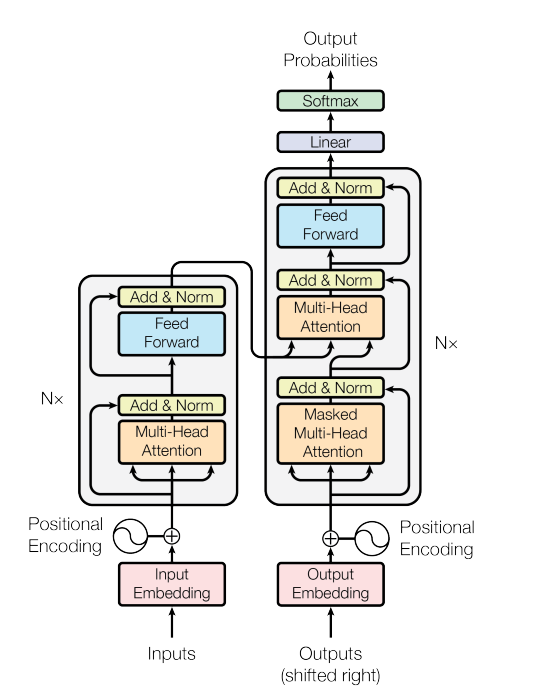
\includegraphics[width=0.5\textwidth]{transformer.png}
  \caption[Architectuur transformer model]{Transformer model architectuur \autocite{VaswaniEtAl2017}}
  \label{fig:transformer-model}
\end{figure}

\subsection{Trainen van LLM's}
\label{sec:trainen-van-llms}
Het trainen van LLM's is een complex proces dat veel tijd en rekenkracht vereist. Dit gebeurt in verschillende stappen.
De eerste fase begint bij het verzamelen van een grote hoeveelheid tekst die gebruikt wordt om het model te trainen.
Deze tekst wordt gehaald uit verschillende artikelen, websites, boeken en andere bronnen. 

Zo kan het volgende woord in een sequentie van tekst voorspeld worden.

Het model krijgt deze grote hoeveelheid tekst in de pre-training fase.
In deze fase leert de LLM grammatica, semantiek, taal patronen en factuele informatie \autocite{Cacic2023}.
Voordat de data meegegeven wordt aan het model moet de data gecleaned en geformatteerd worden.
Dit gebeurt in het tokenization proces. 
Hier wordt de tekst omgezet in tokens die het model kan verwerken \ref{fig:tokenization}.
Woorden kunnen kleiner gemaakt worden zodat de volledige tekst in het model past. 
Dit gebeurt wanneer het model een beperkte input capaciteit heeft \autocite{ElHousieny2023}.
Deze woorden worden dan omgezet wordt in embeddings en deze embeddings worden meegegeven aan het model om het te trainen.
Uit de data kunnen dan patronen gehaald worden met behulp van Transformers \ref{sec:architectuur-van-llms}, maar het is nog niet in staat om vragen of instructies te begrijpen.

\begin{figure}[h]
  \centering
  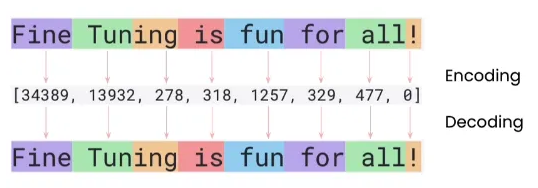
\includegraphics[width=0.5\textwidth]{tokenization.png}
  \caption[Tokenisatie van tekst]{Gesimplificeerde tokenisatie van tekst \autocite{TeeTracker2023}}
  \label{fig:tokenization}
\end{figure}

De volgende fase bestaat uit het trainen van het model op een dataset met instructies en het antwoord erop. 
Volgens \textcite{Das2024} is dit het gesuperviseerde Fine-Tunen van een LLM.
In deze fase probeert het model de patronen te leren die nodig zijn om vragen te beantwoorden of instructies te volgen.
Dit zorgt ervoor dat het model instructies kan volgen en vragen leert te beantwoorden.

Er kan gebruik gemaakt worden om het model specifiek aan de wensen van de mens te laten voldoen. Dit kan door het gebruiken van Reinfocement Learning met menselijke feedback \autocite{LambertEtAL2022}. 
Hierbij geeft de mens feedback aan het model en leert het model bij door deze feedback.

\subsection{Fine-Tuning van LLM's}
\label{sec:fine-tuning-van-llms}

Volgens \textcite{Peckham2024} kan het model achteraf nog extra getraind worden op een specifieke dataset zoals Python code of medische data.
Dit proces heet het Fine-Tunen van een LLM.
Een vereiste voor het Fine-Tunen van een LLM is dat de dataset een grote hoeveelheid data moet hebben.
Ook moet de dataset van hoge kwaliteit zijn en moet de dataset het onderwerp representatief voorstellen \autocite{Peckham2024}.

\subsection{Prompt Engineering}
\label{sec:prompt-engineering}

Prompt Engineering is een techniek die gebruikt wordt om de uitkomst van een LLM te beïnvloeden volgens \textcite{Google2023}.
Er wordt een prompt gegeven aan het model met duidelijke instructies over wat er verwacht wordt. 
Wanneer deze instructies niet voldoen, wordt de prompt iteratief aangepast en wordt de uitkomst geëvalueerd totdat de gewenste uitkomst is bereikt.
Dit iteratieve proces heet Prompt Engineering \autocite{Trad2024}.

Door het toevoegen van enkele voorbeelden aan de prompt kan het model beter begrijpen wat er verwacht wordt \autocite{OpenAi2024a}.
\begin{itemize}
  \item Geef structuur aan de prompt.
  \item Geef een rol mee.
  \item Geef een context.
  \item Geef een doel.
\end{itemize} 
Dit zijn de beste manieren om een prompt te structureren volgens \autocite{Google2023}.

\subsection{Bestaande LLM's}
\label{sec:bestaande-llms}

Momenteel zijn er verschillende LLM's die gebruikt worden voor verschillende taken.
Deze LLM's zijn getraind op verschillende datasets en hebben verschillende architecturen.
Het is belangrijk dat er een duidelijk beeld is van de verschillende LLM's en hun mogelijkheden. 
Met dit beeld kan er een goede keuze gemaakt worden voor het genereren van documentatie.

Eén van de grote spelers in de wereld van LLM's is OpenAI. OpenAI heeft verschillende LLM's ontwikkeld gaande van GPT \autocite{RandfordEtAL2018} tot GPT-4 \autocite{OpenAI2023}.
Het is getraind op een grote hoeveelheid data en heeft een grote capaciteit.
Een nadeel is dat GPT-4 een betalende service is \autocite{OpenAI2023}.

Een andere grote speler is Google. Google heeft verschillende LLM's ontwikkeld waaronder BERT van \textcite{DevlinEtAl2019} en Gemini \autocite{Google2024}.
BERT staat voor Bidirectional Encoder Representations from Transformers, een DL model waar elk output element verbonden is met elk input element \autocite{HashemiPour2024}.
BERT was een eerste stap in de wereld van LLM's voor Google. Sinds kort heeft \textcite{Google2024} een nieuwe LLM ontwikkeld genaamd Gemini.
Deze LLM is een sterke concurrent voor GPT-4 van \textcite{OpenAI2023}. 

Google \autocite{Google2024} bracht een model met verschillende versies uit: Gemini Pro, Gemini Ultra en Gemini Nano. 
Elke versie is gemaakt voor een specifiek doel. Zo is Gemini Nano het meest efficiënte model voor mobiele toestellen, terwijl Gemini Pro het beste model is voor het schalen van allerlei taken.
En Gemini Ultra is het meest capabele en grootste model van Google. Dit kan gebruikt worden voor complexe taken.
Een van de voordelen van Gemini is dat er een groot aantal input tokens meegegeven kunnen worden, namelijk 1 miljoen tokens \autocite{Google2024}.
Dit is aanzienlijk meer dan de 128 duizend tokens van GPT-4.

Een derde speler in de wereld van LLM's is Meta. Meta heeft verschillende LLM's ontwikkeld onder de naam LLama 2 \autocite{Meta2024}.
De LLama 2 familie bestaat uit verschillende LLM's die getraind zijn op verschillende data. Sommige zijn extra getraind voor specifiekere doeleinden.
Zo is er bijvoorbeeld een LLM getraind op Python code, genaamd Code LLama 2 van \textcite{Roziere2024}.
Een voordeel van de LLama 2 familie is dat deze LLM's open sourced zijn en dus voor iedereen toegankelijk zijn.

Antropic heeft ook een LLM ontwikkeld genaamd Claude \autocite{Anthropic2023}. 
Claude's capaciteiten zijn code generatie, het verstaan van meerdere talen, beelden analyseren en kan geavanceerde redeneringen geven.
Er bestaan 3 versies van Claude: Haiku, Sonnet en Opus.
Haiku is een lichte versie van Claude en Sonnet is de combinatie van performantie en snelheid. Opus is het intelligentste model dat complexe taken kan uitvoeren en begrijpen.
Claude is een betalende service en de prijzen zijn afhankelijk van de gekozen versie van Claude \autocite{Anthropic2023}.

De verschillen tussen deze LLM's zijn groot. Zo is er een verschil in capaciteit, trainingsdata en toegankelijkheid.
Het is belangrijk dat er een goede keuze gemaakt wordt voor het genereren van documentatie.
Deze keuze zal afhangen van de mogelijkheden van de LLM's en de doeleinden van de documentatie.

\begin{table}[h!]
\centering
\resizebox{\textwidth}{!}{
\begin{tabular}{|c|c|c|c|c|} 
  \hline
  Model & Input (1M tokens) & Output (1M tokens) & Context & Snelheid (t/s)\\ [0.5ex] 
  \hline
  GPT-4 Turbo \autocite{OpenAi2024} & \$10.00 & \$30.00 &  128k & 18\\ 
  \hline
  GPT-4 \autocite{OpenAi2024} & \$30.00 & \$60.00 &  128k & 21\\ 
  \hline
  GPT-3.5 Turbo \autocite{OpenAi2024} & \$0.50 & \$1.50 &  16k & 52\\
  \hline
  Gemini 1.5 Pro \textcite{Google2024} & \$3.50 & \$10.50 &  128k & 52\\
  \hline
  Code LLama \autocite{Meta2024} & \$0.90 & \$0.90 & 100k & 34\\
  \hline
  LLama 2 \autocite{Meta2024} & \$0.95 & \$1.00 & 100k & 34\\
  \hline
  Claude Opus \autocite{Anthropic2023} & \$15.00  & \$75 &  200k & 29\\
  \hline
  Claude Sonnet \autocite{Anthropic2023} & \$3.00  & \$15 &  200k & 61\\ 
  \hline
  Claude Haiku \autocite{Anthropic2023} & \$0.20  & \$1.20 &  200k & 102\\
  \hline
\end{tabular}}
\caption{Vergelijking van verschillende LLM's op basis van prijs (\$), context (aantal tokens) en snelheid (Tokens per seconde) \autocite{ArtificialAnalysis2024}}
\label{table:vgl-llms}
\end{table}

In de tabel \ref{table:vgl-llms} wordt er een vergelijking gemaakt tussen verschillende LLM's.
Hierin wordt er gekeken naar de prijs van de input en output tokens, de grootte van de context en het aantal tokens dat per seconde verwerkt kan worden.

\begin{table}[h!]
\centering
\resizebox{\textwidth}{!}{
\begin{tabular}{|c|c|c|c|}
\hline
Model & Coding & Beredenering en Kennis\\
\hline
GPT-4 Turbo \autocite{OpenAi2024} & 86\% & 85.4\% \\
\hline
GPT-4 \autocite{OpenAi2024} & 86\% & 88.4\% \\
\hline
GPT-3.5 Turbo \autocite{OpenAi2024} & 70\% & 73.2\% \\
\hline
Gemini 1.5 Pro \textcite{Google2024} & 82\% & 71.9\% \\
\hline
Code LLama \autocite{Meta2024} & /  & 67.8\% \\
\hline
LLama 2 \autocite{Meta2024} & 69\%  & / \\
\hline
Claude Opus \autocite{Anthropic2023} & 87\%  & / \\
\hline
Claude Sonnet \autocite{Anthropic2023} & 79\%  & / \\
\hline
Claude Haiku \autocite{Anthropic2023} & 75\%  & / \\
\hline
\end{tabular}}
\caption{Vergelijking LLM's op basis van beoordeling van menselijke evaluatie en MMLU \autocite{ArtificialAnalysis2024}}
\label{table:vgl-llms-eval}
\end{table}

In de tabel \ref{table:vgl-llms-eval} wordt een vergelijking gemaakt tussen verschillende LLM's tussen twee kolommen. 
De eerste kolom bevat de beoordeling van de coding mogelijkheden van het model gequoteerd met menselijke evaluatie. 
In de tweede kolom staat de quotering op basis van de MMLU een dataset opgesteld door \textcite{Hendrycks2020}.
MMLU staat voor het meten van de multitask taalbegrip capaciteiten van een model \autocite{Hendrycks2020}.
Beide kolommen staan uitgedrukt in procenten met 100\% als maximum.
Hieruit kan geconcludeerd worden dat GPT-4 en GPT-4 Turbo de beste scores behalen op beide vlakken.
Maar omdat er in dit onderzoek gezocht wordt naar een goedkope oplossing wordt er geconcludeerd uit beide tabellen dat GPT-3.5 Turbo de beste prijs/kwaliteit verhouding heeft.

%%=============================================================================
%% Methodologie
%%=============================================================================

\chapter{\IfLanguageName{dutch}{Methodologie}{Methodology}}%
\label{ch:methodologie}

%% TODO: In dit hoofstuk geef je een korte toelichting over hoe je te werk bent
%% gegaan. Verdeel je onderzoek in grote fasen, en licht in elke fase toe wat
%% de doelstelling was, welke deliverables daar uit gekomen zijn, en welke
%% onderzoeksmethoden je daarbij toegepast hebt. Verantwoord waarom je
%% op deze manier te werk gegaan bent.
%% 
%% Voorbeelden van zulke fasen zijn: literatuurstudie, opstellen van een
%% requirements-analyse, opstellen long-list (bij vergelijkende studie),
%% selectie van geschikte tools (bij vergelijkende studie, "short-list"),
%% opzetten testopstelling/PoC, uitvoeren testen en verzamelen
%% van resultaten, analyse van resultaten, ...
%%
%% !!!!! LET OP !!!!!
%%
%% Het is uitdrukkelijk NIET de bedoeling dat je het grootste deel van de corpus
%% van je bachelorproef in dit hoofstuk verwerkt! Dit hoofdstuk is eerder een
%% kort overzicht van je plan van aanpak.
%%
%% Maak voor elke fase (behalve het literatuuronderzoek) een NIEUW HOOFDSTUK aan
%% en geef het een gepaste titel.
\begin{figure}[h]
    \centering
    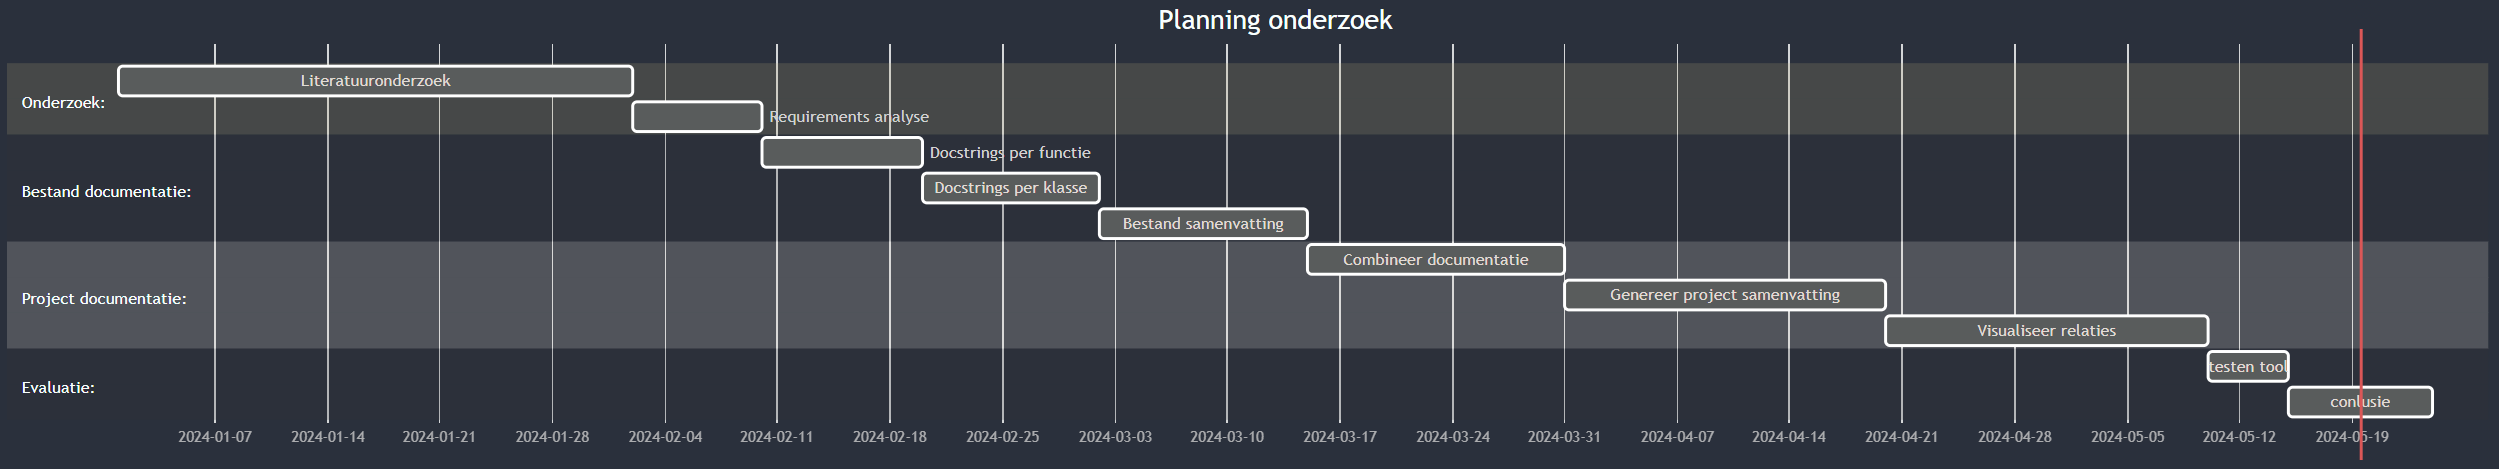
\includegraphics[width=1\textwidth]{flowchart.png}
    \caption{Tijdslijn onderzoek}
    \label{fig:flowchart}
\end{figure}

Het onderzoek is in drie fases opgedeeld. De eerste fase omvat de literatuurstudie.
In deze literatuurstudie wordt er onderzocht wat de huidige stand van zaken is omtent de technologie en mogelijkheden voor de documentatie van Python projecten met behulp van Large Language Modellen.
Zo wordt er gekeken naar wat LLM's zijn, hoe ze werken en wat bestaande tools zijn voor het genereren van documentatie.

Nadat er een duidelijk beeld gevormd is in de literatuurstudie, kan er begonnen worden aan de tweede fase.
Hier wordt er een tool ontwikkeld die een Python bestand kan analyseren en op basis daarvan documentatie kan genereren, aan de hand van het toevoegen van docstrings aan de code.
Dit doet het eerst per functie dan per klasse en uiteindelijk voor het gehele bestand. Dit kan later gebruikt worden om een samenvatting van het project te genereren in de volgende fase.
De uitkomst van deze fase is een tool die de documentatie van een Python bestand kan genereren. 
Door aan prompt engineering te doen, met het prompt dat meegegeven wordt aan de LLM, kunnen de bekomen docstrings accurater worden.
Verder wordt er gekeken naar hoe de documentatie van Python functies gebruikt kan worden voor het maken van een gehele samenvatting van het project.
Dit wordt gedaan op basis van huidige methoden om docstrings aan te maken en te gebruiken. 
Erna kunnen de verschillende docstrings met de bijhorende naam van de functie of klasse gebruikt worden om een samenvatting te genereren.
Deze informatie kan dan gegeven worden aan de Large Language Modellen om een samenvatting te genereren.

De derde fase beslaagt het documenteren van een geheel project.
Door de vorige fases te combineren, het documenteren van de individuele bestanden en het genereren van een samenvatting van het project, kan er een tool gemaakt worden die de documentatie van een geheel project kan genereren.
Deze documentatie bestaat uit de individuele documentatie van de bestanden en een samenvatting van het gehele project. 
Alsook wordt er gekeken naar hoe de relaties tussen de verschillende bestanden gevisualiseerd kunnen worden.

De laatste fase is het evalueren van de tool.
Hier wordt er gekeken naar de kwaliteit van de documentatie die de tool genereert.
Dit wordt gedaan door de documentatie van de tool te vergelijken met de handgeschreven documentatie van een project.
Dit wordt gedaan voor een bestand, een klein project en een groot project.

\section{Requirementsanalyse}
\label{sec:requirements-analyse}
De requirementsanalyse is een belangrijk onderdeel van het onderzoek. 
Hier wordt er gekeken naar wat de tool moet kunnen en wat de verwachtingen zijn van de tool.

\subsection{Functionele requirements}
\label{sec:functionele-requirements}
\subsubsection{Should Have:}
\begin{itemize}
    \item De tool moet in staat zijn om docstrings te genereren voor functies en klassen voor een Python bestand.\\
    De tool genereert docstrings voor functies en klassen in een Python bestand. Dit gebeurt door de code te analyseren en op basis daarvan een docstring te genereren.
    \item De tool moet in staat zijn om een samenvatting van een Python bestand te genereren.\\
    De tool maakt een samenvatting van een Python bestand. In deze samenvatting zitten de belangrijkste zaken van het bestand.
    Zijnde de functies en klassen die erin voorkomen en wat deze doen, alsook hun eventuele parameters en de uitkomst.
    \item De tool moet in staat zijn om een samenhangende samenvatting van een Python project te genereren.\\
    De tool dient een samenvatting te maken van een Python project. Deze samenvatting bestaat uit de individuele samenvattingen van de bestanden en een overkoepelende samenvatting van het project.
    Hierin staan alle functies en klassen die in het project voorkomen en wat deze doen, alsook hun eventuele parameters en de uitkomst.
    \item De tool moet in staat zijn om de relaties tussen de verschillende bestanden van een project te visualiseren.\\
    De tool visualiseert de relaties tussen de verschillende bestanden van een project. Zo is er geweten waar de bestanden naar verwijzen en van waar ze refereren.
\end{itemize}

\subsubsection{Could Have:}
\begin{itemize}
    \item De tool moet in staat zijn om de documentatie van een Python bestand te genereren in verschillende formaten.\\
    De tool genereert de documentatie van een Python bestand in verschillende formaten. Zo kan de gebruiker kiezen in welk formaat hij de documentatie wil.
    \item De tool moet in staat zijn om de relaties tussen de verschillende functies en klassen van een bestand te visualiseren op project niveau\\
    De tool visualiseert de relaties tussen de verschillende functies en klassen van een bestand op project niveau. Zo is er geweten waar de functies en klassen naar verwijzen en van waar ze refereren.
\end{itemize}

\subsubsection{Nice to Have:}
\begin{itemize}
    \item De tool moet in staat zijn om de documentatie van een Python bestand te genereren in verschillende talen.\\
    De tool genereert de documentatie van een Python bestand in verschillende talen. Zo kan de gebruiker kiezen in welke taal hij de documentatie wil.
    \item De tool moet in staat zijn om de documentatie van een Python bestand te genereren in verschillende stijlen.\\
    De tool genereert de documentatie van een Python bestand in verschillende stijlen. Zo kan de gebruiker kiezen in welke stijl hij de documentatie wil.
\end{itemize}

\subsection{Niet-functionele requirements}
\label{sec:niet-functionele-requirements}
\begin{itemize}
    \item De tool moet gebruiksvriendelijk zijn.\\
    De tool moet eenvoudig te gebruiken zijn. Dit betekent dat de tool intuïtief moet zijn en dat de gebruiker geen moeite moet doen om de tool te gebruiken.
    \item De tool moet betaalbaar zijn.\\
    Dit wil zeggen dat de tool geen hoge kosten met zich meebrengt.
    \item De tool moet snel werken.\\
    De tool moet snel werken. Dit betekent dat de tool snel de documentatie moet kunnen genereren. Sneller dan dat een persoon dit zou kunnen.
    \item De tool moet leesbare documentatie genereren.\\
    De documentatie die de tool genereert moet leesbaar zijn. Dit wil zeggen dat de documentatie duidelijk moet zijn en dat de gebruiker er gemakkelijk informatie uit kan halen.    
\end{itemize}

\section{Opstellen van een long-list tools}
\label{sec:long-list}
De long-list bestaat uit de verschillende tools die gebruikt kunnen worden voor het genereren van documentatie voor Pythonprojecten.
Deze tools worden onderzocht en vergeleken om te kijken welke het beste past bij de requirements van de tool.

De oplijsting van de tools is gebaseerd op de literatuurstudie en bestaat uit de volgende tools:
\begin{itemize}
\item Sphinx \autocite{Sphinx2023}\\
Een tool die gebruikt wordt voor het genereren van documentatie voor projecten met reeds een docstring. 
\item Doxygen \autocite{Doxygen2023}\\
Een tool die gebruikt wordt voor het genereren van documentatie voor projecten met reeds een docstring.
\item Pdoc \autocite{GallantHils2023}\\
Een tool die een API genereert voor Python projecten met reeds een docstring.
\item GPT4Docstrings \autocite{Trofficus2023}\\
Een tool die docstrings genereert voor Python projecten met behulp van GPT4 \textcite{OpenAI2023}.
\end{itemize}

Door de verschillende tools te onderzoeken en te vergelijken aan de hand van de requirementsanalyse kan er een keuze gemaakt worden welke tool het beste past bij de requirements van de tool.
Als er geen tool is die voldoet aan de requirements, kan er gekeken worden naar het combineren van verschillende tools of gebruiken van delen van verschillende tools om zo een eigen tool te maken.

Door eerst te kijken naar de programmeerttalen waarvoor de tools gebruikt kunnen worden, kan er al een eerste selectie gemaakt worden uit tabel \ref{table:vgl-tools}.
Zo kan er gekeken worden naar de tools die gebruikt kunnen worden voor Python projecten.
Vervolgens kan er gekeken worden naar het type documentatie dat de tools genereren.
Hierbij kan er gekeken worden naar de tools die docstrings genereren, aangezien dit de basis is voor het genereren van de gewenste documentatie.

\begin{table}[h!]
\centering
\resizebox{\textwidth}{!}{
\begin{tabular}{|c|c|c|c|c|}
\hline
Tool & docstrings & samenvatting bestand & samenvatting project & visualisatie \\ [0.5ex]
\hline
Doxygen & nee & ja & ja & ja \\
\hline
Sphinx & nee & ja & ja & nee \\
\hline
GPT4Docstrings & ja & nee & nee & nee \\
\hline
Pdoc & nee & ja & nee & nee \\
\hline
\end{tabular}}
\caption{Requirementsanalyse van de verschillende tools}
\label{table:ra-tools}
\end{table}

Uit deze tabel \ref{table:ra-tools} kan er geconcludeerd worden dat geen enkele tool voldoet aan de volledige requirements van de tool.
Doordat de Doxygen en Sphinx tools geen docstrings genereren en dit de basis is voor de documentatie, kunnen deze tools niet gebruikt worden.
Pdoc genereert enkel samenvattingen van een bestand dat reeds aangevuld is met docstrings en kan dus ook niet gebruikt worden.
Omdat GPT4Docstrings enkel docstrings genereert en geen samenvattingen van bestanden of projecten, kan er gekeken worden hoe deze tool dit doet.

% Voeg hier je eigen hoofdstukken toe die de ``corpus'' van je bachelorproef
% vormen. De structuur en titels hangen af van je eigen onderzoek. Je kan bv.
% elke fase in je onderzoek in een apart hoofdstuk bespreken.

% ==============================================
% Resultaten
% ==============================================
\chapter{\IfLanguageName{dutch}{Resultaten}{Results}}%
\label{ch:resultaten}

% =================================================================================================
% File Documentation
% =================================================================================================
\section{Bestand documentatie}
\label{sec:bestanddocumentatie}

\subsection{Inleiding}
\label{sec:bestanddocumentatie-inleiding}
In dit hoofdstuk wordt er gekeken naar de documentatie van een Python-bestand.
Eerst wordt de code van het bestand geanalyseerd en worden de verschillende functies en klassen geïdentificeerd.
Op basis van deze functies en klassen worden er docstrings gegenereerd, die opnieuw toegevoegd worden aan de code van het bestand.
Daarna worden de docstrings binnen het bestand gebruikt om een samenvatting van het bestand te genereren.

Deze samenvatting kan dan als basis gebruikt worden voor het genereren van documentatie voor een Python-project, wat bestaat uit een gehele samenvatting en de relaties tussen de verschillende bestanden van het project.
Dit wordt verder onderzocht in het volgende hoofdstuk.
Vooraleer dit kan gebeuren, moet de bestand documentatie op punt staan en geoptimaliseerd worden.

Omdat dit onderzoek een bepaalde scope heeft, is er gekozen om enkel te kijken naar het documenteren van correcte Python-bestanden.
Dit wil zeggen dat er verwacht wordt dat de code correct is en dat er geen syntax fouten in de code zitten.
Er wordt niet gekeken naar het documenteren van bestanden met syntax fouten of bestanden die niet correct zijn.

\subsection{Keuze van model}
\label{sec:bestanddocumentatie-model}

Uit de literatuurstudie is gebleken dat GPT3.5-Turbo van \textcite{OpenAi2024} het beste model is. 
Dit model heeft de beste prijs-kwaliteit verhouding volgens de tabellen \ref{table:vgl-llms-eval} en \ref{table:vgl-llms} van de literatuurstudie.
Dit is een krachtig model dat getraind is op een grote hoeveelheid data en die in staat is om natuurlijke taal te genereren.
Aangezien dit model getraind is op een grote hoeveelheid data is het geschikt om met de juiste prompts de gewenste uitkomst te genereren.


\subsection{GPT4Docstrings tool}
\label{sec:bestanddocumentatie-tool}
Uit de short-list met bestaande tools die voldoen aan de requirements is gebleken dat de tool GPT4Docstrings van \textcite{Trofficus2023} een tool is die het toelaat om docstrings te genereren voor ongedocumenteerde Python-projecten.
Deze tool maakt gebruik van GPT4 \autocite{OpenAI2023} om de docstrings te genereren.
De resultaten van deze tool zijn beoordeeld en geëvalueerd volgens de requirementsanalyse. Een voorbeeld van deze uitkomst is te zien in het codefragment~\ref{lst:gpt4docstrings-uitkomst}.

\begin{listing}
    \caption{Voorbeeld uitkomst van GPT4Docstrings. \autocite{Trofficus2023}}
    \label{lst:gpt4docstrings-uitkomst}
    \begin{minted}{python}
import asyncio
async def async_example():
    """
    An asynchronous example function.

    This function asynchronously sleeps for 2 seconds.

    Returns
    -------
    None
        This function does not return any value.
    """
    await asyncio.sleep(2)
    \end{minted}
\end{listing}

Deze tool is enkel in staat om docstrings te genereren voor functies en klassen.
In deze bachelorproef wordt GPT3.5-Turbo van \textcite{OpenAi2024} gebruikt via Azure van \textcite{Microsoft2024}.
Door het gebruiken van Azure kan de eigen uitgewerkte tool niet vergeleken worden met GPT4Docstrings van \textcite{Trofficus2023} omdat deze een \mintinline{python3}|API_Key| van OpenAi \autocite{OpenAi2024} vereist.
Hierdoor is er gekozen om de technieken, die GPT4Docstrings gebruikt, te implementeren in een eigen tool.
Dit laat toe om de tool uit te breiden en te verbeteren volgens de requirementsanalyse, ook geeft het meer controle over de gegenereerde docstrings.

\subsection{Abstract Syntax Tree}
\label{sec:bestanddocumentatie-ast}
Voor er docstrings gegenereerd kunnen worden, moet er eerst nagegaan worden hoe de code van een Python-bestand geanalyseerd kan worden.
Uit de literatuurstudie is gebleken dat de verschillende functies en klassen in een bestand geïdentificeerd en geëxtraheerd kunnen worden aan de hand van een Abstract Syntax Tree (AST).
Het analyseren van de code van de tool GPT4Docstrings gemaakt door \textcite{Trofficus2023} heeft een beter beeld gegeven hoe een AST eruitziet en hoe deze gegenereerd kan worden.

Een AST is een boomstructuur die de syntactische structuur van een programma weergeeft.
Per knoop in de boom wordt er een deel van de code voorgesteld. 
Deze knoop kan dan weer kinderen hebben die deel uitmaken van de code.
Elke knoop in de boom heeft een type en een waarde.

Het inlezen van een Python-bestand en deze omzetten naar een AST maakt het mogelijk om de code van het bestand te manipuleren.
Zo kunnen de verschillende import statements, functies en klassen geïdentificeerd worden.

\begin{listing}
    \caption[Ophalen functies uit AST]{Voorbeeld van het ophalen van functies uit een AST.}
    \label{lst:ast-voorbeeld}
    \begin{minted}{python}
        def get_functions(self):
            functions = {}
            for node in ast.walk(self.tree):
                if isinstance(node, ast.FunctionDef) or isinstance(node, ast.AsyncFunctionDef):
                    function_code = ast.unparse(node)
                    functions[node.name] = function_code
            return functions
    \end{minted}
\end{listing}

In \ref{lst:ast-voorbeeld} wordt er met behulp van de ast.walk functie door de AST gelopen.
Elke node in de AST wordt gecontroleerd of het een functie of een asynchrone functie is.
Als dit het geval is, wordt de code van de functie opgehaald en toegevoegd aan een dictionary.

\subsection{Docstrings}
\label{sec:bestanddocumentatie-docstrings}
Binnen deze bachelorproef wordt de docstring stijl van Google gehanteerd \autocite{GPT2024}.
Deze docstrings bestaan uit een korte beschrijving van de functie of klasse, de argumenten die de functie verwacht en de return waarde van de functie.
Een voorbeeld van een docstring voor een functie die controleert of een getal een priemgetal is, kan gevonden worden in het codefragment~\ref{lst:docstring-voorbeeld}.

\begin{listing}
    \caption[Docstring van een functie]{Voorbeeld van een docstring voor een functie die controleert of een getal een priemgetal is.}
    \label{lst:docstring-voorbeeld}
    \begin{minted}{python}
    def is_prime(n: int) -> bool:
        """
        Check if a number is prime.

        Args:
            n (int): The number to check.

        Returns:
            bool: True if the number is prime, False otherwise.
        """
    \end{minted}
\end{listing}

Deze docstrings dienen gegenereerd te worden voor elke functie en klasse in een Python-bestand op basis van de huidige code van de functie of klasse.

\subsection{Prompting}
\label{sec:bestanddocumentatie-prompting}

Door aan prompt-engineering te doen, kan het model beter aangestuurd worden en kan de gewenste uitkomst volgens de requirementsanalyse bekomen worden.
Er werden verschillende prompts getest om het beste resultaat te bekomen.
Er zijn prompts gemaakt voor het genereren van docstrings voor functies en klassen. 

\subsubsection{Prompt engineering voor functies}

\begin{listing}
    \caption{Prompt voor het genereren van een docstring voor een functie v1.}
    \label{lst:prompt1}
    \begin{minted}{python}
        '''For this Python function:
        ```python	
        def is_prime(n):
        if n in [2, 3]:
            return True
        if (n == 1) or (n % 2 == 0):
            return False
        r = 3
        while r * r <= n:
            if n % r == 0:
                return False
            r += 2
        return True
        ```
        Leave out any imports, just return the function with the docstring and type hints.
        The function, with docstring using the google docstring style and with type hints is:
        ```python	
        def is_prime(n: int) -> bool:
        """
        Check if a number is prime.
        Args:
            n (int): The number to check.
        Returns:
            bool: True if the number is prime, False otherwise.
        """
        if n in [2, 3]:
            return True
        if (n == 1) or (n % 2 == 0):
            return False
        r = 3
        while r * r <= n:
            if n % r == 0:
                return False
            r += 2
        return True
        ```
        
        For this Python function:
        ```python	
        {code}
        '''
    \end{minted}
\end{listing}

Het eerste prompt voor het genereren van een docstring voor een functie is te zien in het codefragment~\ref{lst:prompt1}.
Er wordt gevraagd om een docstring te genereren voor een functie. Deze versie van de prompt bevat een voorbeeld van een functie met de verwachte uitkomst. 

De volgende versie van dit prompt bevat duidelijkere instructies te vinden in de bijlage \ref{bijlage:prompt2}.
Het is belangrijk dat de prompt duidelijk is en dat het model weet wat er verwacht wordt. 
Daarom staat er in de instructies exact wat er verwacht wordt van het model namelijk dat de gegenereerde functie een docstring moet bevatten en type hints.
De code van de functie mag niet aangepast worden en er mogen geen imports toegevoegd worden.
Ook mag het model niets veronderstellen over de functie of de data types die gebruikt worden in de functie.

Door het vergelijken van de uitkomst, te zien in het codefragment~\ref{lst:uitkomst-prompt2}, met een vooropgestelde uitkomst \ref{bijlage:zelfgedocumenteerd-bestand}, een zelfgedocumenteerd bestand, kan er gekeken worden of de gegenereerde docstrings correct was.
\begin{listing}
    \caption{Uitkomst prompt voor het genereren van een docstring voor een functie v2.}
    \label{lst:uitkomst-prompt2}
    \begin{minted}{python}
    def crop_faces(plot_images: bool=False, max_images_to_plot: int=5) -> List[ndarray]:
    """
    Crop faces from images and save them in a directory.

    Args:
        plot_images (bool, optional): Whether to plot the images. Defaults to False.
        max_images_to_plot (int, optional): Maximum number of images to plot. Defaults to 5.

    Returns:
        List[ndarray]: List of cropped images.
    """
    \end{minted}
\end{listing}
Er wordt geconstateerd dat de uitkomst van het model correct is met uitzondering van de type hints. 
Dit probleem is opgelost door met de volgende versie \ref{bijlage:prompt3} van de prompt de import statements mee te geven.
Zo kan het model geen foute veronderstellingen maken, ook al werd er in de instructies duidelijk meegegeven dat dit niet de bedoeling was.

Deze veronderstellingen kwamen er omdat het model de code van de functie sporadisch aanpaste.
In het aangepaste prompt werd er duidelijk gemaakt dat de uitkomst van de prompt slechts de functienaam met type hint en de docstring moest bevatten.
De code van de functie moest niet meer in de uitkomst staan.

\subsubsection{Prompt engineering voor klassen}
Het prompt engineering proces voor klassen liep gelijkaardig met dat van functies.
Er werd een prompt gemaakt met duidelijke instructies en een voorbeeld van een klasse met de verwachte uitkomst.
De instructies waren gelijkaardig aan die van de functies, maar dan voor klassen.

De verschillende prompt versies 1-4 voor klassen zijn identiek aan die van functies, maar dan met de code van een klasse in plaats van een functie.
Omdat een klasse bestaat uit verschillende functies en attributen is het belangrijk dat de docstrings van de functies en attributen correct gegenereerd worden.
Deze docstrings worden dan meegegeven in de prompt voor het genereren van de docstring van de klasse.
Hiervoor is de overige code van de klasse niet nodig, wat dan ook niet meegegeven wordt in de prompt.
Ook worden opnieuw de verschillende imports meegeven aan de prompt omdat dit hallucinaties vermijdt zoals gezien in hoofdstuk~\ref{sec:bestanddocumentatie-prompting}.
Door de uitkomst, te zien in het codefragment~\ref{lst:uitkomst-prompt4}, van prompt versie 4~\ref{bijlage:prompt4} te vergelijken met een vooropgestelde uitkomst \ref{bijlage:zelfgedocumenteerd-bestand-2} kon er gekeken worden of de gegenereerde docstrings correct waren.
De conclusie hieruit is dat de uitkomst overeenkomt met de vooropgestelde uitkomst. 

\begin{listing}
    \caption{Uitkomst prompt voor het genereren van een docstring voor een klasse v4.}
    \label{lst:uitkomst-prompt4}
    \begin{minted}{python}
    class CsvReader:
    """
    A class representing a CSV file reader with a method to read the file and return its content as a list of rows.

    Methods:
        readCsv: Read a CSV file and return its content as a list of rows.
    """
    \end{minted}
\end{listing}

\subsubsection{Prompt engineering voor samenvatting}
Voor het genereren van een samenvatting van een Python-bestand werd er een prompt gemaakt met de gegenereerde docstrings van de functies en klassen.
De verschillende docstrings werden meegegeven aan de parameter \mintinline{python3}|code_content| en de naam van het bestand aan de parameter 
\mintinline{python3}|filename|.
Het volledige prompt met alle beschrijvingen kan gevonden worden in \ref{bijlage:bestand-samenvatting}.
Door de gekende technieken van prompt engineering gezien in hoofdstuk~\ref{sec:prompt-engineering} te gebruiken kan het model aangestuurd worden.
Er wordt meegegeven wat er verwacht wordt van het model, wat er in de uitkomst moet staan en op basis van welke data de uitkomst gegenereerd moet worden.

\subsection{Toevoegen van gegenereerde docstrings}
\label{sec:bestanddocumentatie-vervangen}
De gegenereerde docstrings worden vervolgens toegevoegd aan de code van de functies en klassen.
Dit gebeurt door de code van de functie of klasse te vervangen door de gegenereerde docstring.
Deze kunnen vastgelegd worden in de AST om dan de AST te gebruiken als de nieuwe code van het bestand.

Omdat de uitkomst van de prompts altijd in de vorm van een string met een omsloten code blok wordt gegeven, zoals te zien in het codefragment~\ref{lst:prompt1}, dient dit verwijderd te worden voor het toegevoegd wordt aan de code van het bestand. 
Dit wordt gedaan door de uitkomst van het model te parsen en de code blokken te verwijderen.
Enkel de gegenereerde docstring samen met de functie of klasse declaratie moet behouden worden.

De eerste versie van de code voor het toevoegen van de docstrings aan de code van de functies en klassen is te zien in het codefragment~\ref{lst:vervangen-v1}.
Door te testen en te evalueren met verschillende Python-bestanden met moeilijkheidsgraden zoals te zien in \ref{table:bestanden} werd er gekeken of de code correct werkte.

\begin{table}[h!]
    \centering
    \resizebox{\textwidth}{!}{
    \begin{tabular}{|c|c|c|}
        \hline
        \textbf{Bestand} & \textbf{Graad} & \textbf{Motivatie} \\[0.5ex]
        \hline
        Een python functie met één functie: \ref{bijlage:makkelijk} & makkelijk & Eén functie \\
        \hline
        Een Python-bestand met verschillende functies: \ref{bijlage:gemiddeld} & gemiddeld &  Meerdere functies \\
        \hline
        Een Python-bestand met functies en klassen: \ref{bijlage:moeilijk} & moeilijk & Functies en klassen \\
        \hline
        Een complex Python-bestand met verschillende functies en klassen en nested functies: \ref{bijlage:extreem-moeilijk} & extreem & Nested functies en klassen \\
        \hline
    \end{tabular}}
    \caption{Aantal functies en klassen in de verschillende Python-bestanden.}
    \label{table:bestanden}
\end{table}

In deze versie wordt er door de AST gelopen en wordt er gekeken of de node een functie of klasse is met de juiste naam. 
Als dit het geval is, wordt de code van de functie of klasse vervangen door de gegenereerde docstring.
Het toevoegen van de docstring wordt gedaan door de nieuwe code van de functie of klasse in de AST te plaatsen op de plaats van de oude code en dan de nieuwe AST te gebruiken als de nieuwe code van het bestand.

\begin{listing}
    \caption[Code voor het vervangen van een docstring]{Vervangen van de code van een functie door de gegenereerde docstring. \ref{bijlage:vervangen-v1}}
    \label{lst:vervangen-v1}
    \begin{minted}{python}
    def replace_functions(self, functions):
        tree = self.tree
        for node in ast.walk(tree):
            if isinstance(node, (ast.FunctionDef, ast.AsyncFunctionDef)) and node.name in functions:
                new_func_def = ast.parse(functions[node.name]).body
                tree.body.insert(tree.body.index(node), new_func_def)        
        self.tree = tree

    \end{minted}
\end{listing}

Deze code werkte niet volledig zoals verwacht. De oude code werd niet verwijderd uit de AST zoals te zien in het codefragment~\ref{lst:uitkomst-vervangen-dubbel}. 
Dit zorgde voor dubbele functies en klassen in de AST waarvan één met docstring en één zonder. Dit werd opgelost door de oude code te verwijderen uit de AST \ref{bijlage:vervangen-v2}.
Alsook werd de code aangepast zodat functies die binnen een klasse gedefinieerd zijn ook vervangen kunnen worden.
Het verwijderen uit de lijst met functies werd ook toegevoegd zodat de functies die al vervangen zijn niet opnieuw vervangen worden.

\begin{listing}
    \caption{Stuk uit uitkomst van het vervangen van de code van een functie \ref{bijlage:uitkomst-gemiddeld}.}
    \label{lst:uitkomst-vervangen-dubbel}
    \begin{minted}{python}
    def crop_image(img, x1, y1, x2, y2):

        def crop_image(img: ndarray, x1: int, y1: int, x2: int, y2: int) -> ndarray:
            """
            Crop the input image to the specified dimensions.

            Args:
                img (ndarray): The input image.
                x1 (int): The starting x-coordinate for cropping.
                y1 (int): The starting y-coordinate for cropping.
                x2 (int): The ending x-coordinate for cropping.
                y2 (int): The ending y-coordinate for cropping.

            Returns:
                ndarray: The cropped image.
            """
            if x1 < 0 or y1 < 0 or x2 > img.shape[1] or (y2 > img.shape[0]):
                img, x1, x2, y1, y2 = pad_img_to_fit_bbox(img, x1, x2, y1, y2)
            return img[y1:y2, x1:x2, :]
    \end{minted}
\end{listing}

Deze versie werkte zoals verwacht voor bestanden met moeilijkheidsgraad makkelijk tot moeilijk, bestanden zonder ingewikkelde structuren zoals nested functies of nested klassen.
De code liep echter vast bij bestanden met een extreme moeilijkheidsgraad.
Hierdoor moest de code opnieuw aangepast worden omdat de gegenereerde docstrings niet altijd correct toegevoegd werden.
Een nadeel van het werken met AST is dat de parent node van nested functies niet opgeslagen worden.
Dit werd opgelost door het vervangen recursief te laten gebeuren, een betere oplossing dan het gebruiken van if else statements het codefragment~\ref{lst:vervangen-v3}.

\begin{listing}
    \caption[Code voor het vervangen van een docstring v2]{Vervangen van de code van een functie door de gegenereerde docstring. \ref{bijlage:vervangen-v3}}
    \label{lst:vervangen-v3}
    \begin{minted}{python}
    def _replace_functions(self, node, functions):
        if isinstance(node, (ast.FunctionDef, ast.AsyncFunctionDef)) and node.name in functions:
            new_func_def = ast.parse(functions[node.name]).body[0]
            new_func_def.body.extend(node.body)
            parent_node = self._get_parent_node(node)
            index = parent_node.body.index(node)
            parent_node.body.remove(node)
            parent_node.body.insert(index, new_func_def)
            functions.pop(node.name)
        for child_node in ast.iter_child_nodes(node):
            self._replace_functions(child_node, functions)
    \end{minted}
\end{listing}

Door de code recursief te laten lopen, kan de code van nested functies en klassen ook vervangen worden.
Door het gebruiken van de parent node van de node die vervangen dient te worden, kan de docstring op de juiste index geplaatst worden.
De nieuwe node wordt toegevoegd aan de parent node en de oude node wordt verwijderd.
Zo kunnen grote Python-bestanden met complexe structuren ook correct vervangen worden.

\subsection{Bestand samenvatting genereren}
\label{sec:bestanddocumentatie-samenvatting}
De laatste stap in het proces van het documenteren van een Python-bestand is het genereren van een samenvatting van het bestand.
Deze samenvatting wordt gemaakt op basis van de reeds gegenereerde docstrings van de verschillende functies en klassen van het bestand.
Het gebruiken van een prompt waar alle docstrings meegegeven worden kan een correcte samenvatting als eindresultaat bekomen.
Hierin hoort er een korte beschrijving van het bestand te staan en een lijst van de functies en klassen die in het bestand voorkomen.
Er komt een beschrijving in de samenvatting van de functies en klassen die in het bestand voorkomen.
Deze beschrijvingen worden gegenereerd door het model op basis van de gegenereerde docstrings.

Deze samenvatting wordt gegenereerd door het model de gegenereerde docstrings van de functies en klassen mee te geven in een prompt, zoals de prompt \ref{bijlage:bestand-samenvatting}.
Dit is de laatste stap in het proces van het documenteren van een Python-bestand.

Deze samenvatting kan dan gebruikt worden als basis voor het genereren van de verdere documentatie voor een Python-project, een samenvatting op project niveau en de relaties tussen de verschillende bestanden van het project.

% \section{LLM voor documentatie}
% \label{sec:llm-voor-documentatie}

% Nadat de basiskennis over LLM's gelegd is, hoe deze werken en wat ze doen. Wat enkele bekende LLM's zijn en wat hun mogelijkheden zijn. 
% Ook zijn er bestaande tools besproken die documentatie genereren voor projecten.

% Omdat dit onderzoek gaat over het documenteren van een Python-project met behulp van LLM's, moet er gekeken worden hoe LLM's gebruikt kunnen worden voor het genereren van documentatie.
% Een LLM kan gebruikt worden voor de verschillende documentatie stukken, samenvattingen, docstrings, relatie tussen de verschillende delen van het project, \dots
% Door de verschillende delen van het project meegegeven aan de LLM met een uitgebreid prompt. 
% Hier kan er telkens aan de Large Language Model gevraagd worden om een samenvatting te maken van wat dit deel van het project doet en wat de uitkomst is.
% Door dit te herhalen voor alle files van het project kan er één samenvattend document gemaakt worden van het gehele project.

% De LLM kan de relaties tussen de verschillende delen van het project leren en vastnemen.
% Zo wordt er een duidelijk beeld gevormd van de structuur van het project en wat de samenhang is van de verschillende delen van het project.
% Alle functies van het Python-project kunnen hier makkelijk teruggevonden worden.

% Er kan ook gebruik gemaakt worden van de LLM om de docstrings van de verschillende functies en klassen te genereren. 
% Om zo een betere samenvatting te verkrijgen van de werking van de verschillende delen van het project, door de docstrings te combineren met de samenvattingen van de LLM.
% Door telkens de docstrings en de naam van de verschillende functies en klassen mee te geven aan de LLM kan er een betere samenvatting gemaakt worden van het gehele project.
% =========================
% Project Documentation
% =========================

\section{Project documentatie}
\label{sec:project-documentatie}

\subsection{Inleiding}
\label{sec:project-documentatie-inleiding}

In dit hoofdstuk wordt er gekeken naar hoe de individuele samenvattingen van een Python bestand gebruikt kunnen worden om een samenvatting van het gehele project te maken.
Alsook wordt er verder gekeken naar hoe de relaties tussen de verschillende bestanden gevisualiseerd kunnen worden.
Dit om een zo goed mogelijk overzicht te krijgen van het project, zonder dat er handmatig documentatie moet worden geschreven.

\subsection{Projectsamenvatting}
\label{sec:project-documentatie-samenvatting}

De samenvatting van een Python project kan gemaakt worden door de individuele samenvattingen van de bestanden samen te voegen.
Deze samenvatting kan bekomen worden door elk python bestand in het project te laten documenteren en de samenvatting ervan op te slaan.
Erna kunnen deze samenvattingen samengevoegd worden om dan mee te geven aan een Large Language Model.
Deze samenvattingen worden gegenereerd door het aanroepen van de functie \mintinline{python3}|generate_file_summaries()|. 
Deze functie maakt gebruik van de klasse \mintinline{python3}|FileDocumenationGenerator()| die de samenvattingen van de bestanden genereerd en opslaat in een dictionary.
De code van deze functie is te vinden in \ref{bijlage:file-summary-functions}.  

Door een duidelijk prompt mee te geven aan het model, kan er specifiek gevraagd worden welke functies en klassen er in het project zitten en dat per bestand duidelijk opgelijst. Samen met deze oplijsting wordt er ook een korte samenvatting van het gehele project weergegeven.
Een voorbeeld van de uitkomst is te zien in \ref{fig:project-summary}.
Hier is te zien dat er een duidelijk overzicht is van welke functies en klassen er in het project zitten, alsook wat het gehele project inhoudt.

\begin{figure}[h]
    \centering
    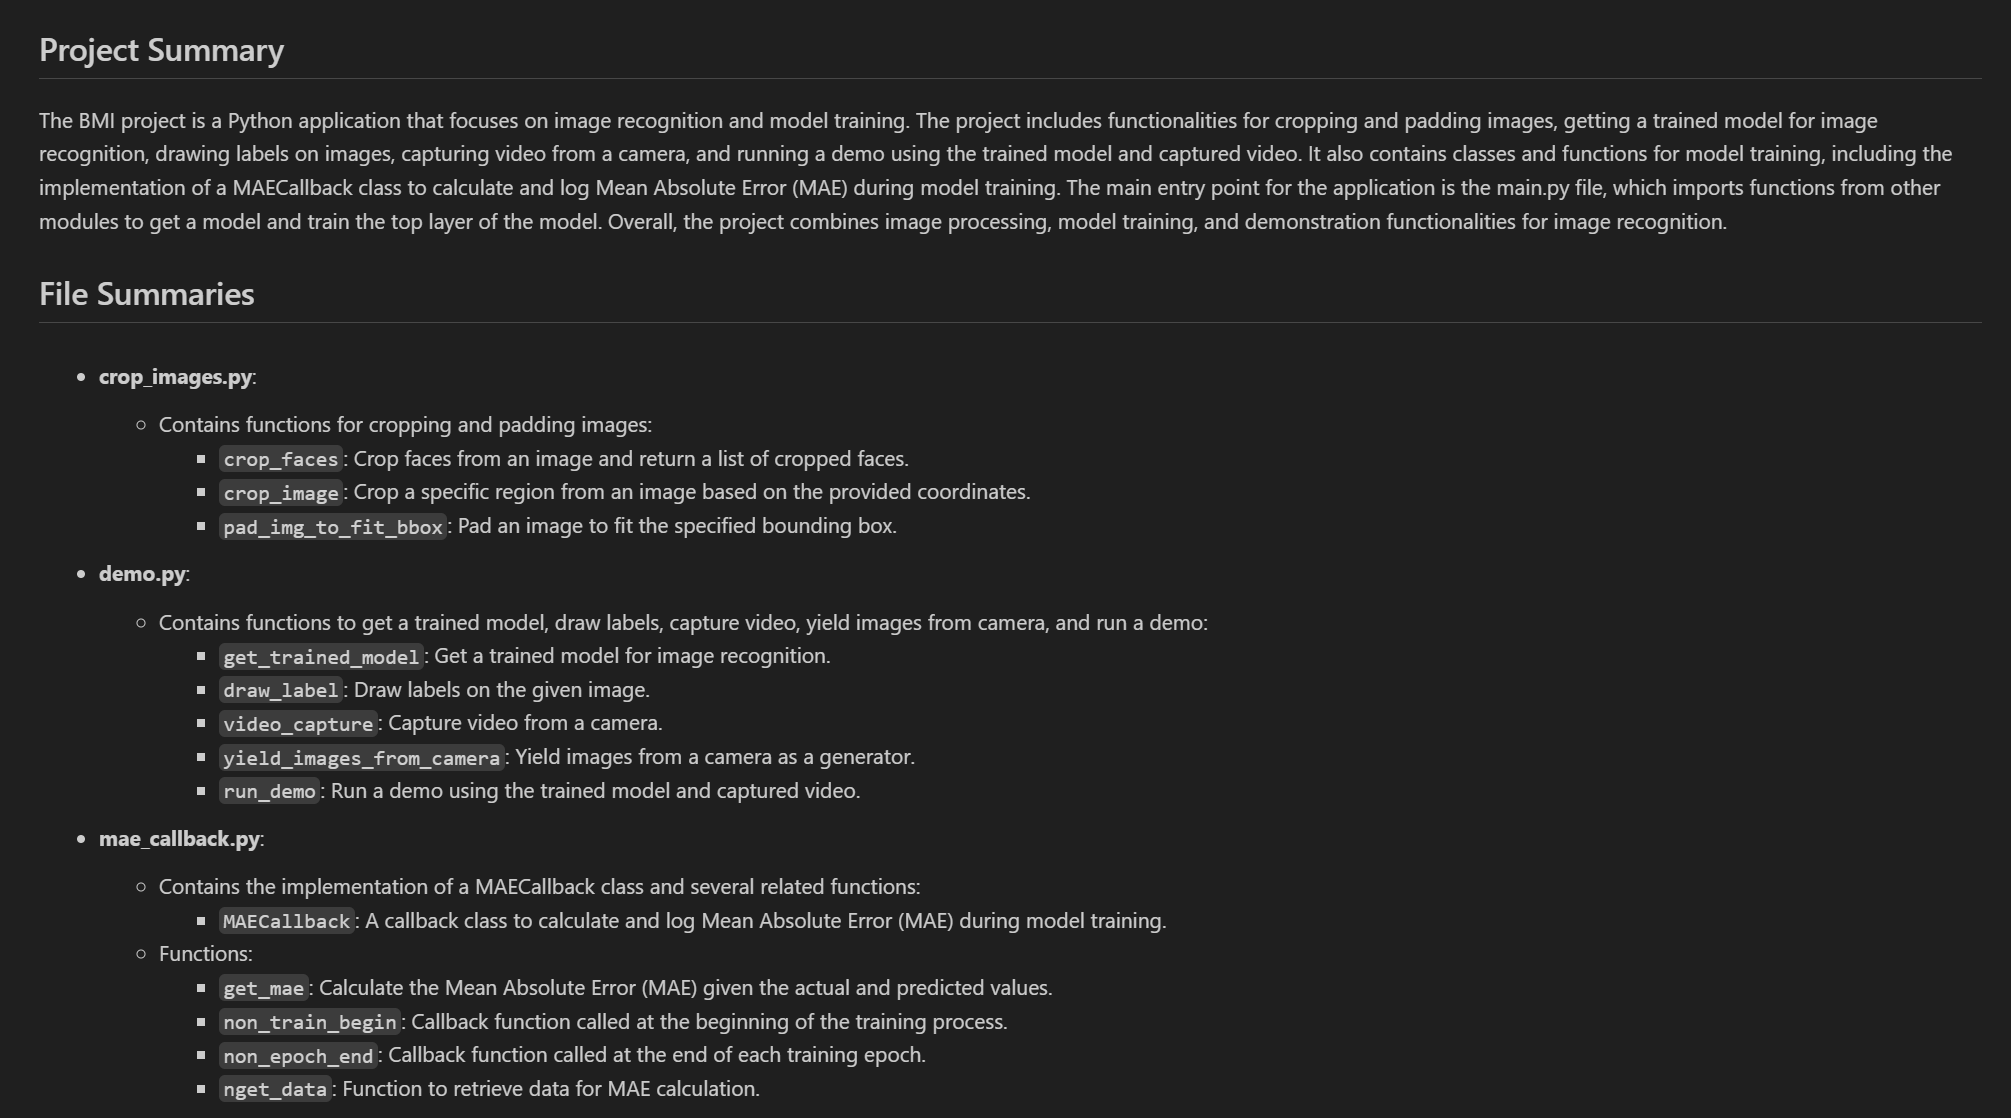
\includegraphics[width=1\textwidth]{project_summary.png}
    \caption{Voorbeeld van een project samenvatting}
    \label{fig:project-summary}
\end{figure}    

\subsubsection{Keuze van welke bestanden te documenteren}
\label{subsec:project-documentatie-keuze-bestanden}

Het is belangrijk om te kijken naar welke bestanden er gedocumenteerd moeten worden.
Omdat het gaat over een Python project, is het belangrijk dat alle Python bestanden gedocumenteerd worden.
Er is de keuze gemaakt om het bestand \mintinline{python3}|__init__.py| niet te documenteren, omdat dit bestand vaak niet relevant is voor de documentatie van het project.
Dit omdat het bestand vaak leeg is of slechts minimale functionaliteit bevat. 
Ook bevat het soms enkele configuratie opties die niet relevant zijn voor de documentatie.

\subsubsection{Documentatie van bestanden zonder functies of klassen}
\label{subsec:project-documentatie-geen-functies}

Omdat er eerst vanuit gegaan wordt dat elk bestand functies of klassen bevat, is het belangrijk om te kijken naar bestanden die dit niet bevatten.
Deze bestanden dienen ook gedocumenteerd te worden om een volledig overzicht te krijgen van het project.
Als er geen apart prompt voorzien wordt dan zal het model hallucineren en een samenvatting verzinnen, dit is niet de bedoeling.
Er is gebruik gemaakt van een prompt \ref{bijlage:bestand-zonder-functies} die vraagt om de werking van het document uit te leggen en de eventuele imports die het bestand bevat.
In dit prompt wordt er duidelijk gedefinieerd wat er in de documentatie moet staan. 
En aan de hand van een voorbeeld wordt er getoond hoe de documentatie eruit moet zien.
Een voorbeeld van de uitkomst in de project documentatie van een bestand zonder functies is te zien in \ref{fig:file-no-functions}.

\begin{figure}[h]
    \centering
    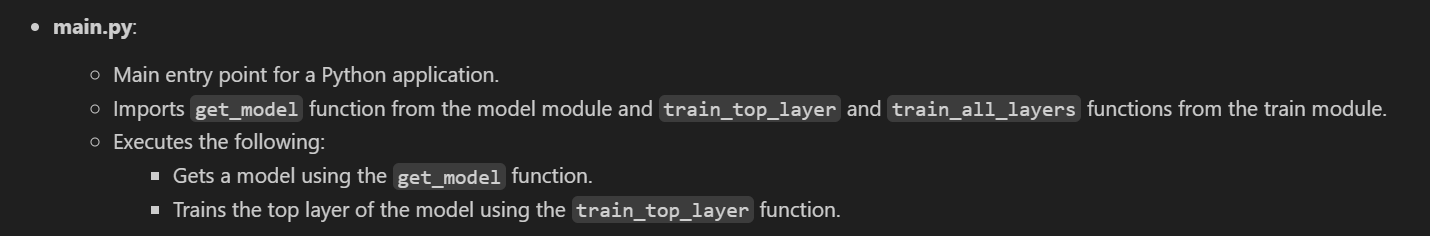
\includegraphics[width=1\textwidth]{documentatie_bestand_zonder_functies.png}
    \caption{Voorbeeld van de documentatie van een bestand zonder functies of klassen}
    \label{fig:file-no-functions}
\end{figure}

\subsubsection{Prompting voor projectsamenvatting}
\label{sec:project-documentatie-prompting}

Aangezien de samenvatting van een project bestaat uit de samenvattingen van individuele Python bestanden, is het belangrijk dat deze op een correcte manier gegenereerd worden.
Dit wordt gerealiseerd met behulp van een prompt die de samenvatting van een Pythonbestand op een correcte manier interpreteert en omzet naar de juiste documentatie.

De gehele samenvatting van het project werd gemaakt door de individuele samenvattingen van de bestanden samen te voegen en dit mee te geven met het prompt \ref{bijlage:prompt6}.
De volgorde van de samenvattingen is niet van belang, omdat de relaties tussen de bestanden later nog gevisualiseerd worden en dit op basis van de imports \ref{sec:project-documentatie-relaties}.
Dit prompt vraagt om de samenvatting van het project te maken en uit de individuele samenvattingen de functies en klassen op te lijsten.

Hierdoor was het niet mogelijk om de gewenste samenvatting te creëren door alle individuele samenvattingen mee te geven aan het model.
Een oplossing die gevonden werd is de volgende: er werden verschillende kleinere prompts meegegeven met het model.
Dit prompt maakt per samenvatting van een Python bestand de documentatie van de verschillende functies en klassen. 
De functies en klassen worden opgelijst met het juiste formaat en een kleine uitleg.
Deze resultaten van de verschillende kleine prompts werden dan code matig samengevoegd tot een geheel. 
Er gaat niets verloren van de individuele samenvattingen, maar om de samenvattingen per bestand met eenzelfde opmaak te krijgen, is deze oplossing gekozen.
Een LLM begrijpt beter een kleiner prompt dan een groot prompt, omdat het model dan beter kan focussen op de vraag en een beter antwoord kan geven.
De uitkomst van de samenvatting van het project is te zien in \ref{fig:project-summary}.

Het prompt dat gebruikt werd is te zien in \ref{bijlage:prompt7}.
Dit prompt vraagt om de functies en klassen van een Python bestand op te lijsten en een korte uitleg te geven van wat deze functies en klassen doen.
De uitkomst is weergegeven met een duidelijk voorbeeld binnen het prompt en volgens een markdown formaat. 
De documentatie genereerd door dit prompt is te zien in \ref{fig:project-summary}.

\subsection{Visualisatie van relaties tussen bestanden}
\label{sec:project-documentatie-relaties}

Om een goed overzicht te krijgen van het project is het belangrijk om de relaties tussen de verschillende bestanden te visualiseren.
Dit kan gedaan worden door gebruik te maken van graven om de relaties tussen de bestanden weer te geven.
Omdat er uit de longlist is gebleken dat er een bestaande tool is die dit kan, namelijk \textcite{Doxygen2023}, is deze tool grondig bekeken.
Voordat Doxygen een visualisatie maakt van de relaties tussen de bestanden vergen deze bestanden grondige documentatie, de relaties tussen de bestanden dienen toegevoegd worden.
Doordat deze tool documentatie vergt, is er gekeken naar hoe deze relaties gegenereerd kunnen worden met behulp van LLM's.
Ook is er gekeken naar hoe Doxygen deze relaties visualiseert, er wordt binnen \textcite{Doxygen2023} gebruikt gemaakt van \textcite{GraphvizAuthors2024}.

\textcite{GraphvizAuthors2024} kan niet gebruikt worden in een Python omgeving, de taal waarin dit onderzoek geschreven is.
Daarom is er gekeken naar een alternatief en soortgelijke tool om de relaties te weergeven.
De tool Pyvis van \textcite{WHIR2018} is een Python library die te gebruiken is om graven te maken en te visualiseren.
Dit laat het toe om de relaties tussen de verschillende bestanden te visualiseren en een duidelijk overzicht te krijgen van het project.

\subsubsection{Genereren van de relaties tussen bestanden in een project}
\label{subsec:project-documentatie-relaties-genereren}

Om de relaties te bekomen tussen alle bestanden en mappen in een project is er een prompt meegegeven aan het Large Language Model.
In dit prompt worden de imports van alle bestanden opgelijst en wordt er gevraagd om de relaties tussen de bestanden weer te geven.
Omdat een bestand dat een functie uit een ander bestand gebruikt deze functie importeerd, staat deze ook tussen de verschillende imports van het bestand.
Hierdoor kan er gekeken worden naar de imports van de verschillende bestanden en zo kunnen de relaties tussen de bestanden worden gevisualiseerd.

Het prompt dat gebruikt werd is te zien in bijlage \ref{bijlage:generate-file-relations}.
Er zijn verschillende iteraties van dit prompt gemaakt om de beste resultaten te bekomen.
Deze iteraties en fouten in het prompt hebben enige tijd in beslag genomen om op te lossen, maar uiteindelijk zijn de kinderziektes eruit gehaald.
Zo is het belangrijk dat er geen spaties in het voorbeeld CSV staan, omdat het model dan niet de het juiste CSV bestand kan genereren.
Ook is het belangrijk dat de imports van de bestanden correct zijn, omdat het model anders niet de juiste relaties kan genereren. 
De uitkomst van dit prompt is een CSV bestand met daarin het pad van het bestand, de bestandsnaam, het pad van de folder waarin het bestand zit en een lijst van alle geimporteerde bestanden.
Omdat dit CSV bestand de basis is voor de graaf die later gemaakt wordt, is het belangrijk dat dit bestand correct is.
Ook zijn schrijffouten en onduidelijkheden in het prompt aangepast om een beter resultaat te bekomen.

Een verdere iteratie van het prompt laat het toe om alle imports in het CSV te laten staan, er wordt achteraf gefilterd op de imports die niet relevant zijn.
Ook is er duidelijk gemaakt aan het prompt dat het bij meerdere imports deze moet opslaan in een lijst gescheiden met een puntkomma.

\subsubsection{Visualisatie van de relaties}
\label{subsec:project-documentatie-relaties-visualisatie}

Eens er een goed CSV bestand is bekomen kunnen de relaties tussen de bestanden gevisualiseerd worden.
Dit wordt gedaan met behulp van de tool Pyvis \autocite{WHIR2018}.
Deze tool haalt de relaties uit het CSV bestand en voegt deze toe aan een graaf. 
Dit door eerst de verschillende nodes toe te voegen en dan de edges tussen de nodes. 
De code waarop dit gebeurt is te vinden in bijlage \ref{bijlage:generate-file-graph}.
Als dit voor alle bestanden gedaan is, kan er een duidelijk overzicht bekomen worden van de relaties tussen de bestanden door de graaf te exporteren naar een HTML bestand.
Dit HTML bestand kan dan geopend worden in een browser om de graaf te bekijken, alsook kunnen de nodes versleept worden om een beter overzicht te bekomen.

\begin{figure}[h]
    \centering
    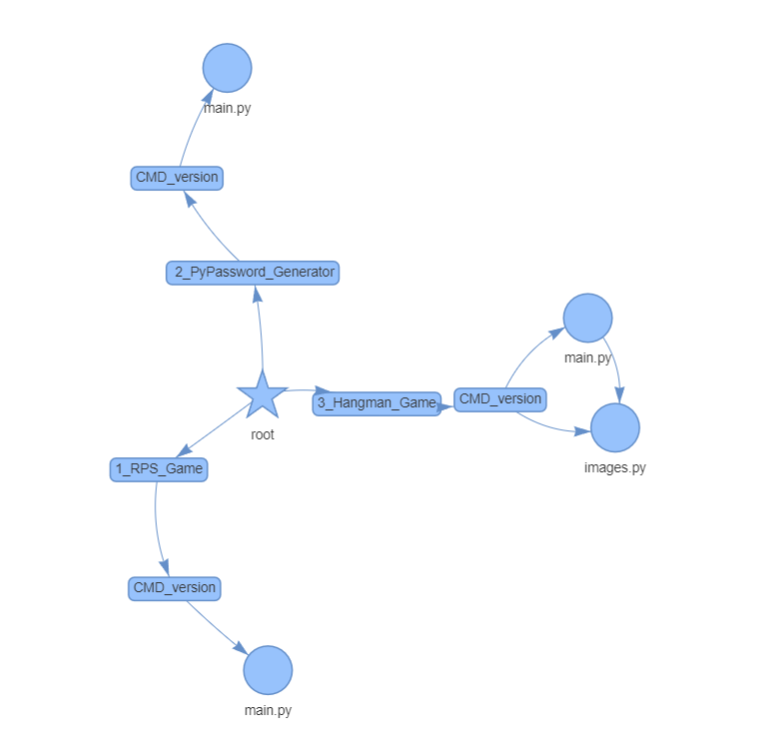
\includegraphics[width=0.5\textwidth]{graph.png}
    \caption{Voorbeeld van een graaf van de relaties tussen bestanden}
    \label{fig:graph}
\end{figure}

Er is een voorbeeld van een graaf te zien in \ref{fig:graph}, alsook is er een voor een groot project een graaf gemaakt om te kijken of de relaties tussen de bestanden duidelijk weergegeven worden op grote schaal \ref{fig:graph-large}.
De relaties op deze graaf zijn zichtbaar echter is het niet altijd duidelijk omdat er veel bestanden zijn en er bepaalde bestanden vaak geïmporteerd zijn.
Dit kan ervoor zorgen dat de graaf onoverzichtelijk wordt met de mate de grote van het projectOpenAi.

\begin{figure}[h]
    \centering
    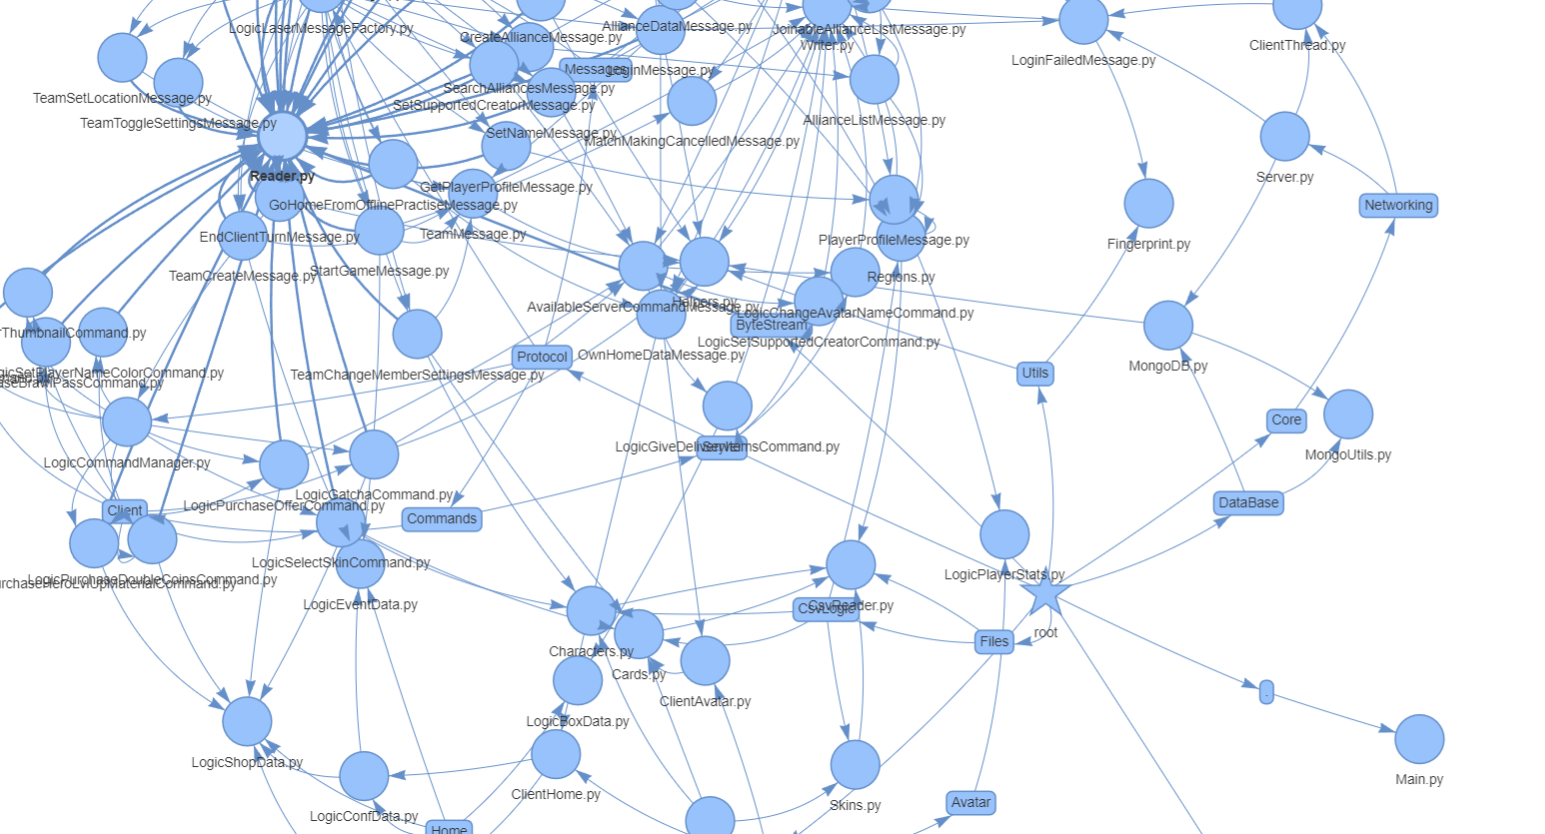
\includegraphics[width=1\textwidth]{graph-large.png}
    \caption{Voorbeeld van een fragment van een graaf van de relaties tussen bestanden van een groot project}
    \label{fig:graph-large}
\end{figure}

\section{Evaluatie}
\label{sec:project-documentatie-evaluatie}

\subsection{Inleiding}
\label{sec:project-documentatie-evaluatie-inleiding}

In dit hoofdstuk wordt er gekeken naar hoe de documentatie van een project geëvalueerd kan worden.
Dit wordt gedaan door de documentatie van de tool te vergelijken met de handgeschreven documentatie van een project.
Dit voor een Python bestand genaamd AutoClicker van \textcite{Waegeneer2022} en een Python project met de naam bmi-project van \textcite{Simmons2019}.

\subsection{Bestanddocumentatie evaulatie}
\label{sec:project-documentatie-evaluatie-bestand}

Door het testen van de moeilijkheidgraden opgesteld in \ref{table:bestanden} kon de tool geëvalueerd worden.
De tool werkte zoals verwacht voor bestanden met moeilijkheidsgraad makkelijk tot moeilijk.
Het vergelijken van de zelfgedocumenteerde bestanden met de automatisch gegenereerde bestanden geeft een goed beeld van de kwaliteit van de gegenereerde docstrings en bestandsamenvattingen.
Wat te zien is in \ref{fig:evaluatie-bestand-documentatie}.
Hieruit is te zien dat de functie omschrijvingen in de samenvatting anders verwoord zijn, maar de betekenis is hetzelfde.
Er is echter één functie die niet gedocumenteerd is manueel, die wel gedocumenteerd is door de tool.
Dit toont aan dat de tool beter presteert dan de programmeur zelf.
Dit is een goed resultaat, omdat de gegenereerde docstrings correct zijn en de samenvatting een correct beeld geeft van het bestand.

\begin{figure}
    \centering
    \begin{subfigure}[b]{1\textwidth}
        \centering
        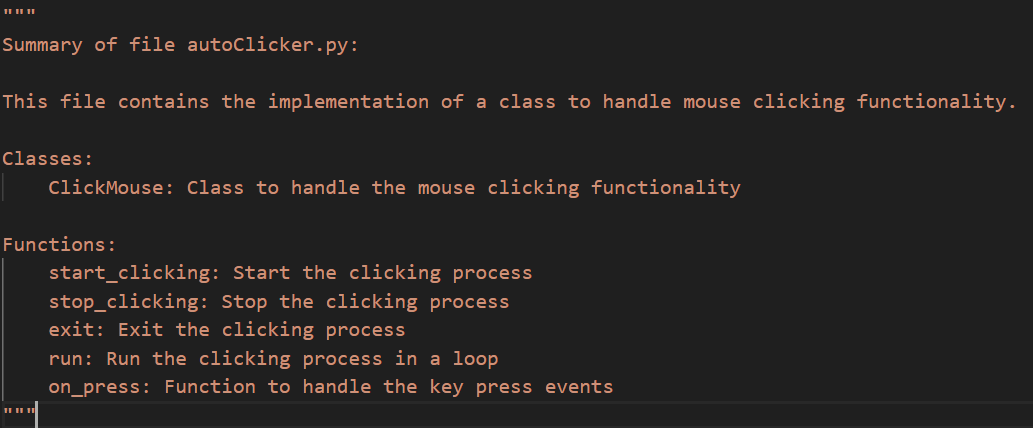
\includegraphics[width=1\textwidth]{zelf_autoclick.png}
        \caption{Zelfgedocumenteerde bestandsamenvatting. \ref{bijlage:zelfgedocumenteerd-bestand}}
        \label{fig:zelfgedocumenteerd-bestandsamenvatting}
    \end{subfigure}
    \hfill
    \begin{subfigure}[b]{1\textwidth}
        \centering
        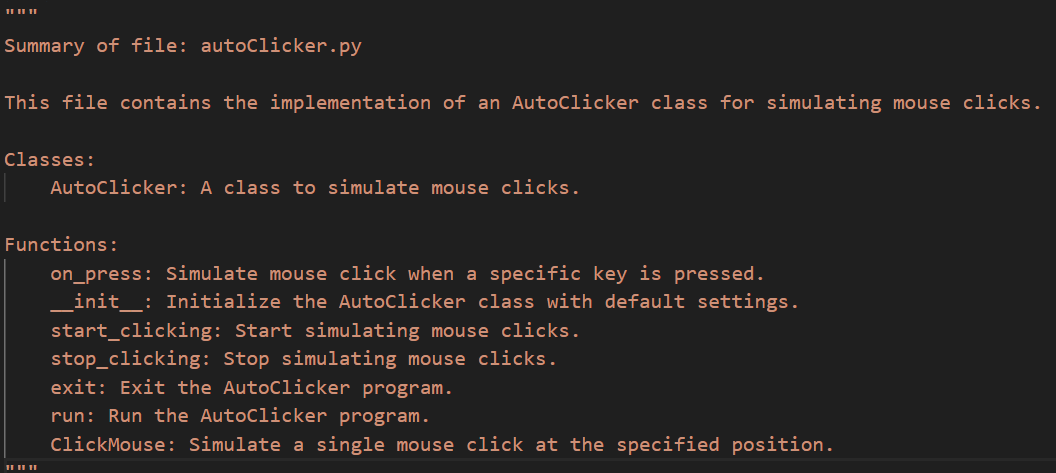
\includegraphics[width=1\textwidth]{automatisch_autoclick.png}
        \caption{Automatisch gegenereerde bestandsamenvatting van eigen tool. \ref{bijlage:evaluatie-bestand-documentatie}}
        \label{fig:automatisch-bestandsamenvatting}
    \end{subfigure}
    \caption{Evaluatie van de automatisch gegenereerde bestandsamenvatting met de zelfgedocumenteerde bestandsamenvatting. Voor het bestand AutoClicker van \textcite{Waegeneer2022}}
    \label{fig:evaluatie-bestand-documentatie}
\end{figure}


\subsection{projectdocumentatie evaluatie}
\label{sec:project-documentatie-evaluatie-project}

Er is een Pythonprojecthandmatig gedocumenteerd, aan dit project zijn de docstrings toegevoegd, samenvattingen per bestand en een samenvatting van het gehele project.
De visualisatie tussen de verschillende bestanden is getekend op papier.

\begin{figure}
    \centering
    \begin{subfigure}[b]{1\textwidth}
        \centering
        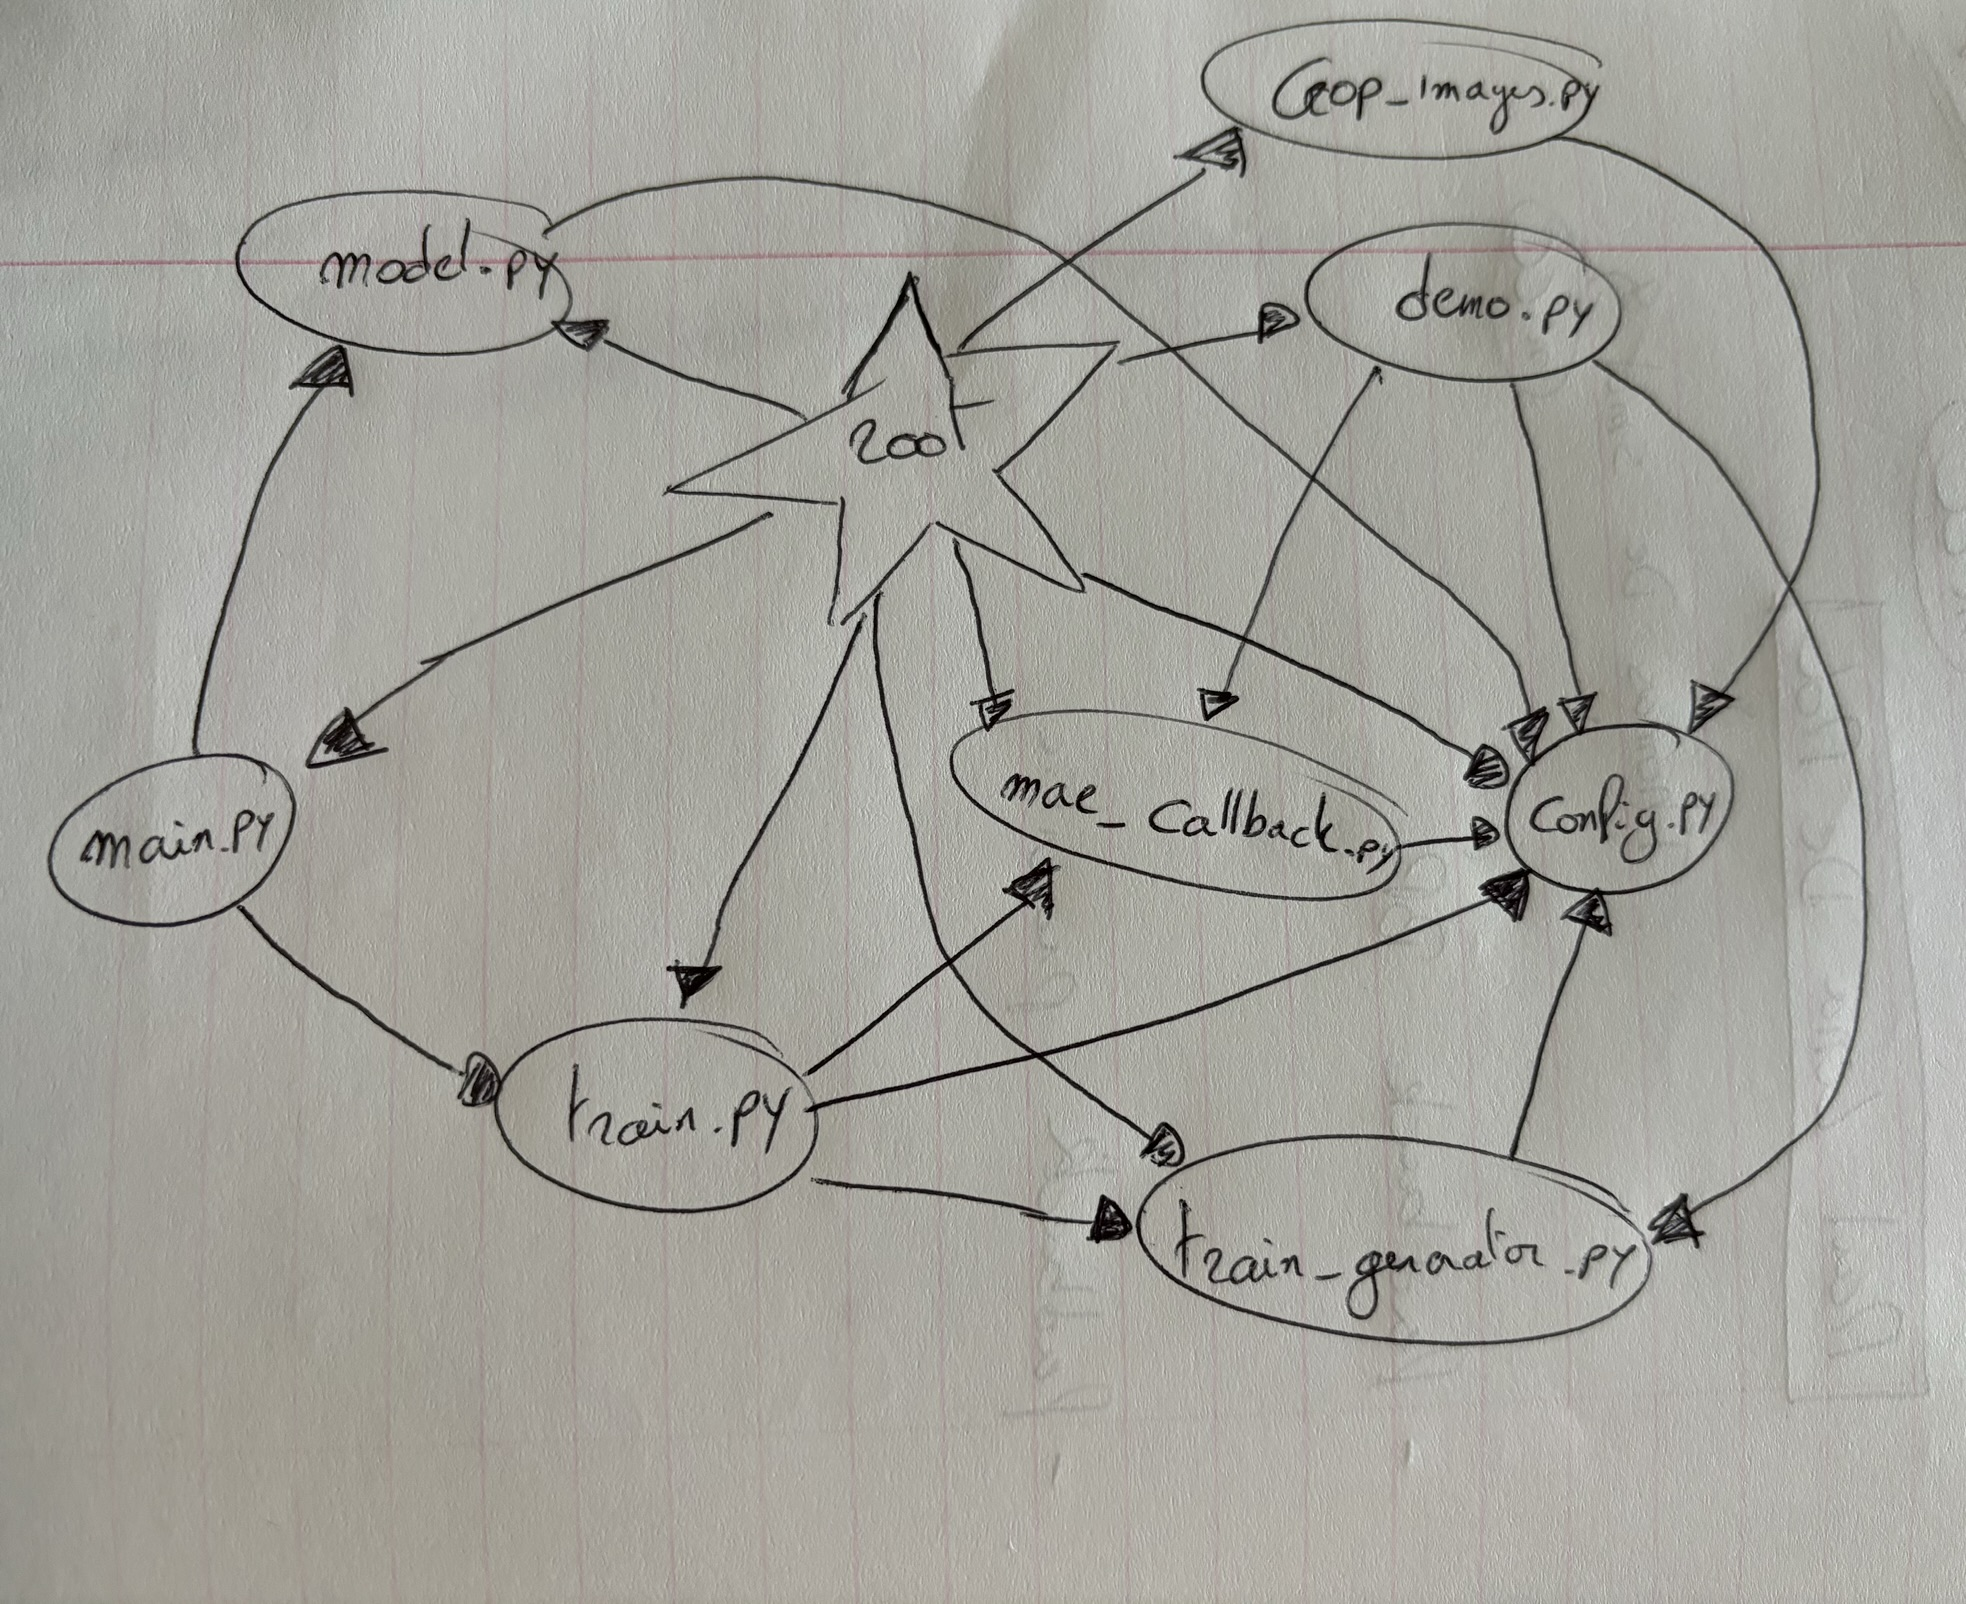
\includegraphics[width=0.5\textwidth]{graaf.png}
        \caption{Handgetekende graaf van de relaties tussen de bestanden van het project \autocite{Simmons2019}}
    \end{subfigure}
    \hfill
    \begin{subfigure}[b]{0.5\textwidth}
        \centering
        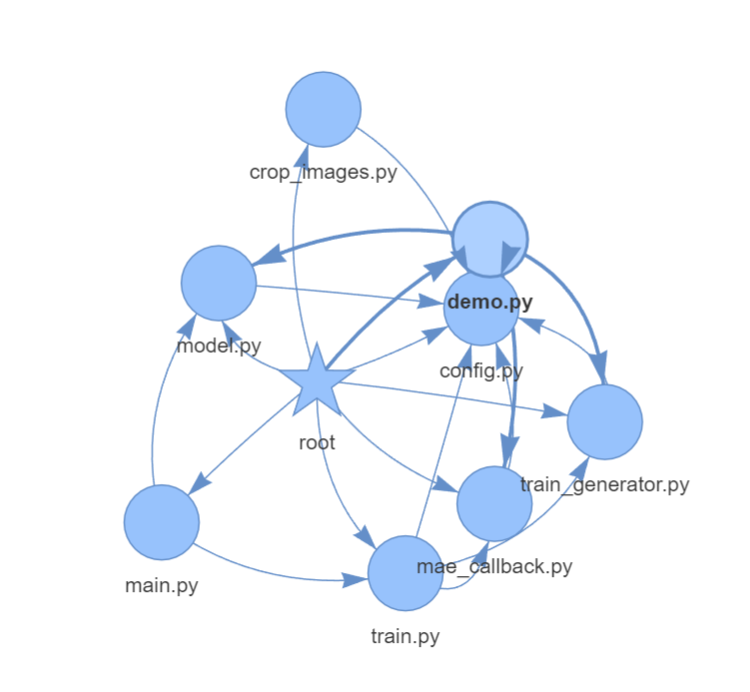
\includegraphics[width=1\textwidth]{generated_graaf.png}
        \caption{Gegenereerde graaf van de relaties tussen de bestanden van het project. \autocite{Simmons2019}}
    \end{subfigure}
    \caption{Vergelijking van de gegenereerde graaf met de handgetekende graaf.}
    \label{fig:evaluatie-graaf}
\end{figure}

De graven te zien in \ref{fig:evaluatie-graaf} tonen de relaties tussen de bestanden van het project. 
Het is duidelijk dat deze graven gelijkaardig zijn, de gegenereerde graaf is beweegbaar en kan aangepast worden om een beter overzicht te krijgen.

Het vergelijken van de samenvattingen en de docstrings laat blijken dat de gegenereerde documentatie correct is.


%\input{...}
%...

%%=============================================================================
%% Conclusie
%%=============================================================================

\chapter{Conclusie}%
\label{ch:conclusie}

% TODO: Trek een duidelijke conclusie, in de vorm van een antwoord op de
% onderzoeksvra(a)g(en). Wat was jouw bijdrage aan het onderzoeksdomein en
% hoe biedt dit meerwaarde aan het vakgebied/doelgroep? 
% Reflecteer kritisch over het resultaat. In Engelse teksten wordt deze sectie
% ``Discussion'' genoemd. Had je deze uitkomst verwacht? Zijn er zaken die nog
% niet duidelijk zijn?
% Heeft het onderzoek geleid tot nieuwe vragen die uitnodigen tot verder 
%onderzoek?

Het onderzoek had als doel de vraag te beantwoorden: "Hoe kan geautomatiseerde documentatiegeneratie met behulp van een Large Language Modellen (LLM) effectief worden toegepast op ongedocumenteerde Pythonprojecten om er duidelijke en overzichtelijke documentatie van te maken?"
Hiervoor werd er een tool ontwikkeld die voldeed aan de requirements die werden opgesteld in het onderzoek.
Enkele van deze requirements zijn dat de tool docstrings kan genereren dat er een bestand- en een projectsamenvatting gegenereerd kan worden en dat de tool zo goedkoop mogelijk moet zijn.
Voor deze vraag beantwoord kan worden is het belangrijk om te weten wat er juist bedoelt wordt met documentatie.
Onder documentatie wordt er begrepen dat er per bestand docstrings en een samenvatting van het bestand worden gegenereerd.
Voor een project wordt er een samenvatting van het project gegenereerd en een overzicht van alle bestanden in het project in de vorm van een graaf met de relaties.

Ook is het belangrijk om te weten wat enkele bestaande documentatietools zijn.
Tools zoals Sphinx, Doxygen en Pdoc zijn in staat om een gedocumenteerd project om te zetten in een website of API.
Deze tools zijn echter niet in staat om ongedocumenteerde projecten te documenteren.
Vervolgens werd de tool GPT4Docstrings besproken, deze tool is in staat om docstrings te genereren voor Pythonprojecten, de code van GPT4Docstrings werd gebruikt in de ontwikkeling van de tool.

Het documenteren van een bestand gebeurt door de code van het bestand in te lezen en per functie of klasse een docstring te genereren.
Vervolgens worden deze docstrings samengevoegd tot een bestandssamenvatting.
Voor een project te documenteren worden de verschillende bestanden in het project gedocumenteerd, worden de bestandssamenvatting samengevoegd tot een projectsamenvatting en wordt er een graaf gegenereerd met de relaties tussen de bestanden.

Er werd gekozen om een Large Language Model te gebruiken om de documentatie te genereren omdat deze modellen getraind zijn op grote hoeveelheden data en zowel code als natuurlijke taal kunnen begrijpen en genereren.
Door het gebruiken van GPT3.5-Turbo werd de tool zo goedkoop mogelijk gehouden.

Door de automatische gegenereerde documentatie van een project te evalueren met een vooropgesteld manueel gedocumenteerd project, werd er gekeken naar de verschillen en overeenkomsten tussen de documentatie van de tool en de handgeschreven documentatie.
De resultaten van de evaluatie tonen aan dat de documentatie van de tool en de handgeschreven documentatie gelijkaardig zijn.
Alhoewel er enkele fouten in de documentatie van de individuele bestanden zitten, blijft de gehele projectdocumentatie overzichtelijk en duidelijk.

Een verdere evaluatie van de tool kan gebeuren door een grote groep programmeurs verschillende projecten handmatig te laten documenteren en dit te chronometreren. 
Dezelfde projecten kunnen dan ook automatisch gedocumenteerd worden met de tool, de snelheid van de tool kan dan vergeleken worden met de snelheid van de programmeurs.
Daarna kan er een enquête afgenomen worden waarbij de programmeurs de keuze hebben tussen de handmatig gedocumenteerde projecten en de automatisch gedocumenteerde projecten.
Deze evaluatie kan dan gebruikt worden om de tool te verbeteren.



% % =============================

% Aangezien dit onderzoek een beperkte scope heeft, zijn er enkele uitbreidingen die kunnen worden toegevoegd om het onderzoek te verbeteren.
% Deze uitbreidingen kunnen helpen om de resultaten van het onderzoek te verbeteren en om de tool verder te ontwikkelen.

% Zo kan er gekeken worden naar het genereren van documentatie voor andere programmeertalen.
% Deze bachelorproef focust zich op Python, maar het is mogelijk om de tool uit te breiden naar andere programmeertalen.
% Aangezien een Large Language Model zoals GPT \autocite{OpenAi2024} ook getraind zijn op andere programmeertalen.

% Ook kan er gekeken worden naar hoe projecten met syntax fouten of andere problemen gedocumenteerd kunnen worden.
% Dit is belangrijk omdat de tool nu enkel werkt op projecten die correcte syntax hebben.
% Deze fouten kunnen eruit gehaald worden door de code eerst door een linter te halen en dan pas de documentatie te genereren.
% De bekomen syntax fouten kunnen dan meegegeven worden aan een model om zo een bestand te genereren zonder syntax fouten.

% Een andere uitbreiding is kijken naar hoe de documentatie geëvalueerd kan worden.
% Omdat dit nu slechts manueel gebeurt, op basis van gezond verstand. 
% Er kan gekozen worden om enquêtes af te nemen bij programmeurs om zo de documentatie te evalueren.
% De evaluatie van de respondenten gaat echter slechts relatief zijn, omdat de respondenten beoordelen op basis van kennis van de programmeertaal. 
% Of er kan gekeken worden naar hoe de documentatie van de tool vergeleken kan worden met de documentatie van de programmeur zelf.
% Hier is het belangrijk om te kijken naar de verschillen en overeenkomsten tussen de documentatie van de tool en de documentatie van de programmeur.

% Een laatste voorbeeld van een uitbreiding is om te kijken naar hoe verschillende Large Language Models presteren op het genereren van documentatie.
% Zo kan er gekozen worden tussen modellen zoals GPT-4 \autocite{OpenAI2023}, LLama 2 \autocite{Meta2024}, Gemini \autocite{Google2024}, \dots

% Sommige modellen hebben een groter context window dan andere modellen, zo zou er meer informatie meegegeven kunnen worden aan het model.
% En het zou mogelijk een beter resultaat kunnen geven.

%---------- Bijlagen -----------------------------------------------------------

\appendix

\chapter{Onderzoeksvoorstel}

Het onderwerp van deze bachelorproef is gebaseerd op een onderzoeksvoorstel dat vooraf werd beoordeeld door de promotor. Dat voorstel is opgenomen in deze bijlage.

%% TODO: 
\section{Samenvatting}

% Kopieer en plak hier de samenvatting (abstract) van je onderzoeksvoorstel.
\begin{abstract}
    Documentatie van een Python project is belangrijk, maar het is een tijdrovende taak en het wordt vaak niet grondig gedaan.
    Deze bachelorproef aan de HoGent onderzoekt het automatisch genereren van documentatie voor python projecten met behulp van Large Language Modellen.
    Er wordt een tool ontwikkeld die de Python code en de relaties tussen de verschillende bestanden analyseert en op basis daarvan een overzichtelijke documentatie genereerd.
    Er wordt gekeken naar hoe de documentatie van Python functies gebruikt kunnen worden voor het maken van een gehele samenvatting van het project.
    Dit wordt gedaan op basis van huidige methoden om docstrings aan te maken en te gebruiken.
    Deze informatie kan dan gegeven worden aan de Large Language Modellen om een samenvatting te genereren.
    
    Er worden verschillende Python projecten verzameld en geanalyseerd om te kijken hoe de documentatie gegenereerd kan worden.
    Dan worden er LLMs getraind op basis van deze projecten en wordt er gekeken naar hoe de documentatie gegenereerd kan worden.
    De gegenereerde documentatie kan dan vergeleken worden met de huidige documentatie van de projecten om dit te evalueren.
    Ook zal er gevraagd worden aan enkele programmeurs om de documentatie te evalueren.
    
    Op basis van deze feedback kan het model gefinetuned worden. Er kan gekeken worden naar de mogelijke verbeteringspunten zodat er uiteindelijk een betere documentatie van het project ontstaat.
    Het resultaat is dat er een tool is die de documentatie van een Python project kan genereren.
    Dit resultaat maakt het mogelijk om de gegenereerde samenvatting van een Python project te lezen. 
    De lezer kan dan stukken gebruiken uit het project of er verder mee aan de slag gaan.
\end{abstract}

% Verwijzing naar het bestand met de inhoud van het onderzoeksvoorstel
%---------- Inleiding ---------------------------------------------------------

\section{Introductie}%
\label{sec:introductie}

Documentatie is belangrijk wanneer er aanpassingen moeten gebeuren aan de code van een project. Ook moet een iemand anders de code kunnen begrijpen voordat de code gebruikt kan worden binnen een ander project.
Hoe kan geautomatiseerde documentatiegeneratie met behulp van Large Language Modellen (LLM) effectief worden toegepast om een duidelijk overzichten en informatieve beschrijvingen te produceren voor Python projecten?

Het is belangrijk dat de skill of de knowhow van een project gedeeld kan worden met anderen. 
Door het toepassen van documentatie kan deze kennis makkelijk vergaard worden door andere geïnteresseerden.
Het is dus een belangrijk dat er aan documentatie gedaan wordt en dat deze up-to-date blijft. 

Documentatie is iets dat veel tijd kost, dat vaak niet gemaakt wordt en het is iets dat up-to-date gehouden moet worden.
Het gebruiken ervan kan ervoor zorgen dat er geen dubbel werk gedaan moet worden. Een tool die dit proces kan versnellen / automatiseren zou een grote meerwaarde zijn.
De tool bestaat uit een geautomatiseerde documentatie LLM die de project code analyseert en samenvat in een document. 
Dit geeft de werknemers de moegelijkheid om zich in te lezen in het project en erna zelf aanpassingen te maken of stukken code te gebruiken voor een ander project.

Het eindresultaat van deze bachelorproef is een Proof of Concept (PoC) van een geautomatiseerde tool die de project code analyseert en er documentatie van genereert.
De gegenereerde documentatie laat het toe om het project te begrijpen zonder er te veel tijd aan te besteden.

%---------- Stand van zaken ---------------------------------------------------

\section{Literatuurstudie}%
\label{sec:Literatuurstudie}

Wat is documentatie binnen Python projecten en wat zijn de huidige tools?
Voor de taal Python bestaan er al verschillende tools die documentatie genereren voor blokken code zoals pdoc \autocite{GallantHils2023} en Sphinx \autocite{Sphinx2023}. 
Met behulp van de sphinx autodoc functie \autocite{Sphinx2023} kan een python functie omschreven worden in een docstring.
Een docstring is een blok tekst dat de werking van een python functie omschrijft. Door deze beknopte blok tekst wordt er duidelijk wat de functie doet.
Deze docstrings kunnen mogelijks gebruikt worden bij het maken van een document dat het project omschrijft.

Er is ook al onderzoek gedaan naar het automatisch genereren van documentatie van code blokken met behulp van een Neural Attention Model (NAM) \autocite{IyerEtAl2016}.
Dit onderzoek heeft gekeken naar het genereren van hoogstaande samenvattingen van source code. 
Het maakt gebruik van neurale netwerken die stukken C\# code en SQL queries omzetten naar zinnen die de code omschrijven. 
Dit helpt bij het begrijpen van stukken code maar niet van een geheel project waar meerdere bestanden bij betrokken zijn.

Hoe kunnen Large Language Modellen gebruikt worden om documentatie te genereren?
Large Language Modellen zijn neurale netwerken die getraind worden op grote hoeveelheden tekst. 
Deze modellen kunnen tekst genereren op basis van een gegeven input. De mogelijkse invoer in deze bachelorproef kan dan een python project zijn, of de docstrings van verschillende functies in een project.
Er wordt dan verwacht dat het een samenvatting maakt van het project of van de functies.

Ook kan er gekeken worden naar GitHub README.md bestanden. Dit zijn bestanden waarin de werking van een project kort wordt uitgelegd. Deze zijn echter niet altijd makkelijk te lezen. 
Volgens de studie \textcite{GaoEtAl2023} kan de tekst vereenvoudigd worden terwijl steeds de correcte betekenis te behouden, en dit aan de hand van een transfer learning model.
Het gebruik van LLMs en het automatisch code documentatie met behulp van syntax bomen wordt onderzocht in \textcite{Procko2023} voor de C\# en .NET programeertalen.
In deze studie wordt er gekeken naar het gebruik van LLMs specifiek GPT-3.5 en GPT-4 om code te documenteren.

In de studie van \textcite{McBurneyMcMillan2014} wordt onderzocht hoe er automatisch documentatie gegenereerd kan worden voor Java code, specifiek naar hoe de methodes met elkaar verbonden zijn en welke rol ze spelen binnen het project.
Dit is een mooi voorbeeld van wat ik wil bereiken met deze bachelorproef, een samenhangend geheel van verschillende bestanden van een python project die samen een duidelijk overzicht geven van de werking van het project.
Hoe kunnen LLMs gebruikt worden om automatisch documentatie te genereren voor python projecten.
De gegenereerde samenvatting van het gehele project geeft de lezer ervan de mogelijkheid het project te gebruiken of aan te passen zonde de totale project code te ontleden.

%---------- Methodologie ------------------------------------------------------
\section{Methodologie}%
\label{sec:methodologie}

Hier beschrijf je hoe je van plan bent het onderzoek te voeren. Welke onderzoekstechniek ga je toepassen om elk van je onderzoeksvragen te beantwoorden? 
Gebruik je hiervoor literatuurstudie, interviews met belanghebbenden (bv.~voor requirements-analyse), experimenten, simulaties, vergelijkende studie, risico-analyse, PoC, \ldots?

Valt je onderwerp onder één van de typische soorten bachelorproeven die besproken zijn in de lessen Research Methods (bv.\ vergelijkende studie of risico-analyse)? 
Zorg er dan ook voor dat we duidelijk de verschillende stappen terug vinden die we verwachten in dit soort onderzoek!

Vermijd onderzoekstechnieken die geen objectieve, meetbare resultaten kunnen opleveren. 
Enquêtes, bijvoorbeeld, zijn voor een bachelorproef informatica meestal \textbf{niet geschikt}. 
De antwoorden zijn eerder meningen dan feiten en in de praktijk blijkt het ook bijzonder moeilijk om voldoende respondenten te vinden. 
Studenten die een enquête willen voeren, hebben meestal ook geen goede definitie van de populatie, 
waardoor ook niet kan aangetoond worden dat eventuele resultaten representatief zijn.

Uit dit onderdeel moet duidelijk naar voor komen dat je bachelorproef ook technisch voldoen\-de diepgang zal bevatten. 
Het zou niet kloppen als een bachelorproef informatica ook door bv.\ een student marketing zou kunnen uitgevoerd worden.

Je beschrijft ook al welke tools (hardware, software, diensten, \ldots) je denkt hiervoor te gebruiken of te ontwikkelen.

Probeer ook een tijdschatting te maken. Hoe lang zal je met elke fase van je onderzoek bezig zijn en wat zijn de concrete \emph{deliverables} in elke fase?

%---------- Verwachte resultaten ----------------------------------------------
\section{Verwacht resultaat, conclusie}%
\label{sec:verwachte_resultaten}

Hier beschrijf je welke resultaten je verwacht. Als je metingen en simulaties uitvoert, kan je hier al mock-ups maken van de grafieken samen met de verwachte conclusies. 
Benoem zeker al je assen en de onderdelen van de grafiek die je gaat gebruiken. 
Dit zorgt ervoor dat je concreet weet welk soort data je moet verzamelen en hoe je die moet meten.

Wat heeft de doelgroep van je onderzoek aan het resultaat? Op welke manier zorgt jouw bachelorproef voor een meerwaarde?

Hier beschrijf je wat je verwacht uit je onderzoek, met de motivatie waarom. Het is \textbf{niet} erg indien uit je onderzoek andere 
resultaten en conclusies vloeien dan dat je hier beschrijft: het is dan juist interessant om te 
onderzoeken waarom jouw hypothesen niet overeenkomen met de resultaten.



%%---------- Andere bijlagen --------------------------------------------------
% TODO: Voeg hier eventuele andere bijlagen toe. Bv. als je deze BP voor de
% tweede keer indient, een overzicht van de verbeteringen t.o.v. het origineel.
% ==========================================
% Bijlage
% ==========================================

\chapter{Bijlage}
\label{bijlage}

In deze bijlage worden de volledige code van de applicatie en de gebruikte prompts weergegeven.

\section{Prompts}
\label{bijlage:prompts}

\subsection{Function Prompt 1}
\label{bijlage:prompt1}
Instructies voor het genereren van een docstring voor een functie versie 1.
\begin{minted}{python}
    '''For this Python function:
    ```python	
    def is_prime(n):
    if n in [2, 3]:
        return True
    if (n == 1) or (n % 2 == 0):
        return False
    r = 3
    while r * r <= n:
        if n % r == 0:
            return False
        r += 2
    return True
    ```
    Leave out any imports, just return the function with the docstring and type hints.
    The function, with docstring using the google docstring style and with type hints is:
    ```python	
    def is_prime(n: int) -> bool:
    """
    Check if a number is prime.
    Args:
        n (int): The number to check.
    Returns:
        bool: True if the number is prime, False otherwise.
    """
    if n in [2, 3]:
        return True
    if (n == 1) or (n % 2 == 0):
        return False
    r = 3
    while r * r <= n:
        if n % r == 0:
            return False
        r += 2
    return True
    ```
    
    For this Python function:
    ```python	
    {code}
    '''
\end{minted}

\subsection{Function Prompt 2}
\label{bijlage:prompt2}
Instructies voor het genereren van een docstring voor een functie versie 2.
\begin{minted}{python}
'''
    The following Python function is a code snippit from a Python file. 
    The following function lacs a docstring and type hints.
    Your task is to add a docstring and type hints to the function.
    You can't change the function's code, add any imports, or assume anything about the function's behavior or datatypes that is not clear from the code snippet itself.
    Below is a function that needs a docstring and type hints:
    ```python	
    def is_prime(n):
    if n in [2, 3]:
        return True
    if (n == 1) or (n % 2 == 0):
        return False
    r = 3
    while r * r <= n:
        if n % r == 0:
            return False
        r += 2
    return True
    ```
    The correct outcome should be the following Python code:
    ```python	
    def is_prime(n: int) -> bool:
    """
    Check if a number is prime.
    Args:
        n (int): The number to check.
    Returns:
        bool: True if the number is prime, False otherwise.
    """
    if n in [2, 3]:
        return True
    if (n == 1) or (n % 2 == 0):
        return False
    r = 3
    while r * r <= n:
        if n % r == 0:
            return False
        r += 2
    return True
    ```
    
    Now it's your turn to add a docstring and type hints to the following function:
    ```python	
    {code}
    ```
    '''
\end{minted}


\subsection{Function Prompt 3}
\label{bijlage:prompt3}
Prompt versie 3 voor het genereren van een docstring voor een functie. 
\begin{minted}{python}
    '''You are an AI documentation assistant, and your task is to generate docstrings and typehints based on the given code of a function, the function is a code snippet from a Python file.
    Do your task with the least amount of assumptions, you can't add any imports, change the code, or assume anything about the function's behavior or datatypes that is not clear from the code snippet itself.
    The purpose of the documentation is to help developers and beginners understand the function and specific usage of the code.

    An example of your task is as follows:
    The given code is:

    ```python	
    def is_prime(n):
    if n in [2, 3]:
        return True
    if (n == 1) or (n % 2 == 0):
        return False
    r = 3
    while r * r <= n:
        if n % r == 0:
            return False
        r += 2
    return True
    ```

    The expected output of your task for the given code is:

    ```python	
    def is_prime(n: int) -> bool:
    """
    Check if a number is prime.

    Args:
        n (int): The number to check.

    Returns:
        bool: True if the number is prime, False otherwise.
    """

    if n in [2, 3]:
        return True
    if (n == 1) or (n % 2 == 0):
        return False
    r = 3
    while r * r <= n:
        if n % r == 0:
            return False
        r += 2
    return True
    ```

    Now it's your turn to generate the docstrings and typehints for the following function of a file with these imports:
    {imports}

    The content of the code is as follows:
    {code_content}
    '''
\end{minted}

\subsection{Class Prompt 1}
\label{bijlage:prompt4}
Prompt voor het genereren van een docstring voor een klasse.
\begin{minted}{python}
    '''
    You are an AI documentation assistant, and your task is to generate docstrings and typehints based on the given code of a class, the class is a code snippet from a Python file.
    Do your task with the least amount of assumptions, you can't add any imports, change the code, or assume anything about the classes behavior or datatypes that is not clear from the code snippet itself.
    The purpose of the documentation is to help developers and beginners understand the function and specific usage of the code.

    An example of your task is as follows:
    The given code is:

    ```python
    class Circle:
        def __init__(self, radius: float) -> None:
            """
            Initialize the Circle object with a given radius.

            Args:
                radius (float): The radius of the circle.
            """
            self.radius = radius

        def calculate_area(self) -> float:
            """
            Calculate the area of the circle.

            Returns:
                float: The area of the circle.
            """
            return round(math.pi * self.radius ** 2, 2)

        def calculate_circumference(self) -> float:
            """
            Calculate the circumference of the circle.

            Returns:
                float: The circumference of the circle.
            """
            return round(2 * math.pi * self.radius, 2)
    ```

    The expected output of your task for the given code is:

    ```python
    class Circle:
        """
        A class representing a circle with methods to calculate its area and circumference.

        Attributes:
            radius (float): The radius of the circle.

        Methods:
            __init__: Initialize the Circle object with a given radius.
            calculate_area: Calculate the area of the circle.
            calculate_circumference: Calculate the circumference of the circle.
        """
    ```

    Now it's your turn to generate the docstrings and typehints for the following class of a file with these imports:
    {imports}

    The content of the code is as follows:
    {code_content}

    Only generate the class docstring

    '''
\end{minted}

\subsection{Samenvatting van een bestand}
\label{bijlage:bestand-samenvatting}
Prompt voor het genereren van een samenvatting van een bestand.
\begin{minted}{python}
    '''
    You are an AI documentation assistant, and your task is to generate a summary of the given Python file. 
    The summary should include the following information:
    - What the file does.
    - What classes are defined in the file.
    - What functions are defined in the file.
    - And a brief description of each class and function.
    - Include the file name at the beginning of the summary.
    
    You are going to generate the summary based on given function names, class names and their docstrings.
    
    Now it's your turn to generate the summary given the following code of the file: {filename}:

    {code_content}
    '''
    \end{minted}

\subsection{Bestand zonder functies of klasses}
\label{bijlage:bestand-zonder-functies}
Prompt voor het genereren van een samenvatting van een bestand zonder functies of klasses.
\begin{minted}{python}
    '''
    You are an AI documentation assistant, and your task is to generate a summary of the given Python file based on the code content.
    The summary should include the following information:
    - What the file does.
    - What is the purpose of the file.
    - What is the main functionality of the file.
    - What the output is
    - What it does when executed.
    - Include the file name at the beginning of the summary.

    An example of the output of your task is as follows:
    Given the following code content:

    ```python
    from model import get_model
    from train import train_top_layer, train_all_layers
    if __name__ == '__main__':
        model = get_model()
        train_top_layer(model)
    ```

    The expected output of your task for the given code is the summary of the file:
    
    ```python
    """
    Summary of file: main.py
    
    This file contains the main functionality for a Python application.
    It imports the get_model function from the model module and the train_top_layer and train_all_layers functions from the train module.
    When executed, it gets a model using the get_model function and trains the top layer of the model using the train_top_layer function.
    """
    ```

    You are going to generate the summary based on the given code content of the file with filename: {filename}.
    {code_content}
    '''
\end{minted}

\subsection{Project samenvatting}
\label{bijlage:prompt6}
Prompt voor het genereren van een samenvatting van een project.
\begin{minted}{python}
    '''
    You are an AI documentation assistant, and your task is to generate a summary of the given Python project.
    The summary should include the following information:
    - What the project does.
    - What files are included in the project. And what each file does. What functions and classes are defined in each file.
    - A brief description of each class and function.
    - Include the project name at the beginning of the summary.

    You are going to generate the summary based on summaries of each file in the project.
    
    Now it's your turn to generate the summary given the following project structure:
    {project_name}

    With the following folder structure:
    {folder_structure}

    And the following summaries of each file:
    {summaries}
    '''
\end{minted}

\subsection{Project samenvatting per file}
\label{bijlage:prompt7}
Prompt voor het genereren van een samenvatting van een project per bestand.
\begin{minted}{python}
'''
    You are an AI documentation assistant, and your task is to generate a markdown summary of a file.
    For the following file summary:
    """
    Summary of file: crop_images.py

    This file contains the implementation of functions for cropping and padding images.

    Functions:
        crop_faces: Crop faces from an image using a specified bounding box.
        crop_image: Crop a specified region from an image.
        pad_img_to_fit_bbox: Pad an image to fit a specified bounding box.
    """

    The output should be:
    - **crop_images.py**: 
        - Contains functions for cropping and padding images:
          - `crop_faces`: Crop faces from an image using the given bounding boxes.
          - `crop_image`: Crop a specific region from an image based on the provided coordinates.
          - `pad_img_to_fit_bbox`: Pad an image to fit the specified bounding box.

    You are going to generate the markdown summary for the file: {file} with the following summary:
    {summary}
    '''
\end{minted}


\section{Code}
\label{bijlage:code}

\subsection{Bestand Documentatie}
\label{bijlage:documentatie-bestand}

\subsubsection{Vervangen van de code van een functie door de gegenereerde docstring. v1}
\label{bijlage:vervangen-v1}
\begin{minted}{python}
def replace_functions(self, functions):
    tree = self.tree
    for node in ast.walk(tree):
        if isinstance(node, (ast.FunctionDef, ast.AsyncFunctionDef)) and node.name in functions:
            new_func_def = ast.parse(functions[node.name]).body
            tree.body.insert(tree.body.index(node), new_func_def)        
    self.tree = tree
\end{minted}

\subsubsection{Vervangen van de code van een functie door de gegenereerde docstring. v2}
\label{bijlage:vervangen-v2}
Versie 2 van de functie om de code van een functie te vervangen door de gegenereerde docstring.
\begin{minted}{python}
def replace_functions(self, functions):
    tree = self.tree
    for node in ast.walk(tree):
        if isinstance(node, ast.ClassDef):
            for child_node in node.body:
                if isinstance(child_node, (ast.FunctionDef, ast.AsyncFunctionDef)) and child_node.name in functions:
                    new_func_def = ast.parse(functions[child_node.name]).body[0]
                    new_func_def.body.extend(child_node.body)
                    idx = node.body.index(child_node)
                    node.body.insert(idx, new_func_def)
                    node.body.remove(child_node)
                    functions.pop(child_node.name)
        elif isinstance(node, (ast.FunctionDef, ast.AsyncFunctionDef)) and node.name in functions:
            new_func_def = ast.parse(functions[node.name]).body[0]
            new_func_def.body.extend(node.body)
            tree.body.insert(tree.body.index(node), new_func_def)
            tree.body.remove(node)
            functions.pop(node.name)
    self.tree = tree
\end{minted}

\subsubsection{Vervangen van de code van een functie door de gegenereerde docstring. v3}
\label{bijlage:vervangen-v3}
\begin{minted}{python}
def _replace_functions(self, node, functions):
    if isinstance(node, (ast.FunctionDef, ast.AsyncFunctionDef)) and node.name in functions:
        new_func_def = ast.parse(functions[node.name]).body[0]
        new_func_def.body.extend(node.body)
        parent_node = self._get_parent_node(node)
        index = parent_node.body.index(node)
        parent_node.body.remove(node)
        parent_node.body.insert(index, new_func_def)
        functions.pop(node.name)
    for child_node in ast.iter_child_nodes(node):
        self._replace_functions(child_node, functions)
\end{minted}

\subsubsection{Genereren van de relaties tussen de verschillende bestanden}
\label{bijlage:generate-file-relations}

\begin{minted}{python}
'''
    You are an AI documentation assistant, and your task is to generate a csv file containing the relations between the files in a Python project.

    For the given project structure and imports:
    The imports are as follows:
    '1_RPS_Game\\CMD_version\\main.py': 'import random', '2_PyPassword_Generator\\CMD_version\\main.py': 'import random', '3_Hangman_Game\\CMD_version\\images.py': '', '3_Hangman_Game\\CMD_version\\main.py': 'import requests\nimport random\nimport os\nfrom images import hangman_logo\nfrom images import stages', '4_Hangman_Game\\CMD_version\\stages.py': '', '4_Hangman_Game\\CMD_version\\images.py': 'import csv\nimport matplotlib', '4_Hangman_Game\\CMD_version\\main.py': 'import random\nimport os\nfrom images import stages\nfrom images import logo'

    The structure of the project is as follows:
    '.': ['LICENSE', 'README.md'], '1_RPS_Game': [], '1_RPS_Game\\CMD_version': ['1_RPS_Game\\CMD_version\\main.py'], '2_PyPassword_Generator': [], '2_PyPassword_Generator\\CMD_version': ['2_PyPassword_Generator\\CMD_version\\main.py'], '3_Hangman_Game': [], '3_Hangman_Game\\CMD_version': ['3_Hangman_Game\\CMD_version\\images.py', '3_Hangman_Game\\CMD_version\\main.py'], '4_Hangman_Game': [], '4_Hangman_Game\\CMD_version': ['4_Hangman_Game\\CMD_version\\stages.py', '4_Hangman_Game\\CMD_version\\images.py', '4_Hangman_Game\\CMD_version\\main.py']

    The expected output of your task is the following:
    ```csv
File_Path,File_Name,Folder_Path,Uses_File
1_RPS_Game\CMD_version\main.py, main.py,1_RPS_Game\CMD_version,[]
2_PyPassword_Generator\CMD_version\main.py,main.py, 2_PyPassword_Generator\CMD_version,[]
3_Hangman_Game\CMD_version\images.py,images.py,3_Hangman_Game\CMD_version,[]
3_Hangman_Game\CMD_version\main.py, main.py,3_Hangman_Game\CMD_version,['3_Hangman_Game.CMD_version.images']
4_Hangman_Game\CMD_version\stages.py,stages.py,4_Hangman_Game\CMD_version,[]
4_Hangman_Game\CMD_version\images.py,images.py,4_Hangman_Game\CMD_version,[]
4_Hangman_Game\CMD_version\main.py,main.py,4_Hangman_Game\CMD_version,['4_Hangman_Game.CMD_version.images';'4_Hangman_Game.CMD_version.stages']
    ```

    The Column "Uses File" should only contain the files where the file imports functions from.
    For example if the imports are:
    ```python
    Import csv
    Import matplotlib
    from images import open_image
    from stages import stage1
    ```
    The Column "Uses File" should contain the file '4_Hangman_Game\\CMD_version\\images.py' and '4_Hangman_Game\\CMD_version\\stages.py'
    Do your task given the following imports and structure of the project:
    
    The imports are as follows:
    {imports}

    And the structure of the project is as follows:
    {structure}

    THE OUTPUT SHOULD BE A SINGLE CSV FILE CONTAINING THE RELATIONS BETWEEN THE FILES IN THE PROJECT.
    '''
\end{minted}

\section{Project Documentatie}

\subsection{Functies voor het samenvatting van een bestand}
\label{bijlage:file-summary-functions}
\begin{minted}{python}
    def document_file(self, file_path, outfolder_path):
        FDG = FileDocumenationGenerator(self.api_key, self.azure_endpoint, file_path, self.folder_path, outfolder_path)
        FDG.generate_file_documentation()
        return FDG

    def generate_file_summaries(self, python_files):
        for file in python_files:
            print("Documenting file: ", file)
            FDG = self.document_file(file, outfolder_path=self.outfolder)
            self.summaries[file] = FDG.get_summary()
            self.imports[file] = FDG.get_imports()
\end{minted}


%%---------- Backmatter, referentielijst ---------------------------------------

\backmatter{}

\setlength\bibitemsep{2pt} %% Add Some space between the bibliograpy entries
\printbibliography[heading=bibintoc]

\end{document}
